% sections/appendix-measurement.tex -- Appendix A, measurement records.
% Writer: B. Written 2026-11-21, from 06:19 UTC (clock: date -u); end time in fix-list-B.md.
% Word count: not budgeted (appendix); one or two sentences per float plus captions.
% Macros used that are not in outline section 7: none.
% Pending labels used: \PendSegLogpTwoLevel.
% Floats placed here (23; tables have bodies floats/<file>.tex holding the tabular only, caption and label here, except
%   tab:exclusions, whose tabular is written below because the outline gives it to writer B):
%   tab:wer-strata, tab:gridshift, tab:headlines (table*), tab:drift, fig:rank, tab:rank-odds, fig:love, tab:balance
%   (table*), fig:classes, tab:nonspeech, tab:vp (table*), fig:tolerance, tab:tolerance, tab:bridge-verdicts, fig:bland,
%   fig:sensitivity, tab:sensitivity, tab:kinds, tab:nonlanguage, tab:labelflips, tab:exclusions (table*), tab:entry,
%   tab:cor. These include the P7 moves of outline section 10 (tab:gridshift, tab:headlines, tab:bridge-verdicts, tab:vp,
%   fig:tolerance, tab:kinds, fig:love); their pointer sentences are in sections 3, 5 and 6.
% Fourth review round (from 12:50 UTC; clock: date -u): fig:bridge and fig:bland removed and tab:bridge-verdicts
%   reduced to verdicts (privacy review P1, P7; methods review M10); fig:rank in two classes per rank (P3); Table B
%   without the other group's medians and the roster-vintage row (P2, P6); census in recordings and the set-aside count
%   as one count (P4); D4's isolated-segment counts withdrawn from Table U and Table D (P7); the precision check without
%   a band (M4, P8).
% Pre-publish verification (2026-11-21, from 21:30 UTC; clock: date -u): the other group and the seen bridge pairs are
%   not counted (\NOtherCreators and \BridgeSeenPairs are text); Table B and the Love plot drop group differences that
%   rest on fewer than 5 creators off the group's common value; Rec. of tab:labelflips under the nested-count rule;
%   a read-precision share of tab:entry resting on fewer than 5 creators is withheld.
% Builder notes: the body of tab:bridge-verdicts must not print the outlying pair's own disagreement, nor a ratio from
%   which it follows; creator counts that fall fewer than 5 short of a printed total are printed as "all but <5" by the
%   builder (second review round, 2026-11-21, 08:25 UTC).
% Literal numerals left in the text are thresholds or constants of method: 5 creators, 1--4, 0.25 and 0.1 (fixed lines),
%   0.2 SD (margin), 0--20% (injection grid), ranks 1--5 and 6--20, 120 days (R4 window), 15 s, 30 s, 60 s, 3 s.

\section{Measurement records}
\label{app:measure}

Every float in this appendix is exploratory (registry A2/A7) and not a test of H1--H10. Text-derived figures come from
the seen creators; counts, durations, dates and languages cover all creators. Cells of fewer than 5 creators are merged
by the plan's rule, and no minimum or maximum of a transcript measure is printed. Moved here from Sections 3 and 5 by
the page limit, unchanged (move log of the third review round): the census flow figure, the paragraphs ``Three levels''
and ``Dates'', the artefact table, the figure of coverage by position, and parts of Sections 5.5 and 5.7.

% Moved here from Section 3 by the page limit (third review round); caption unchanged.
\begin{figure*}[tp]
\centering
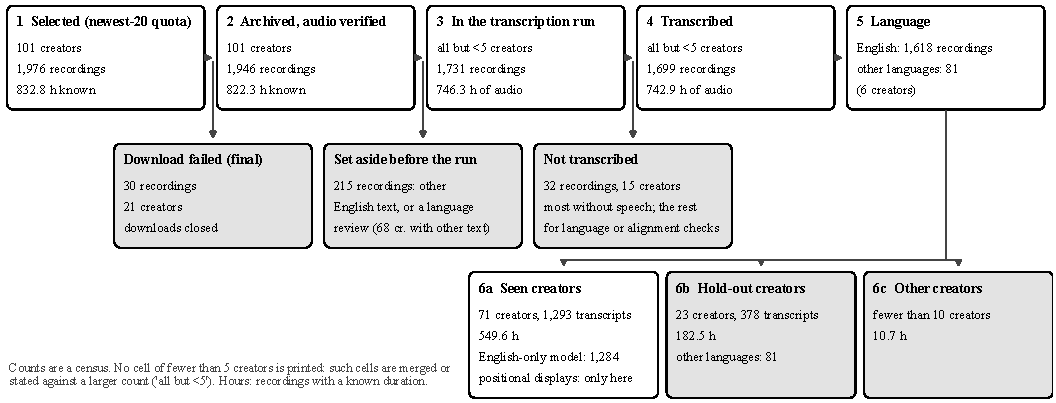
\includegraphics[width=\textwidth]{floats/fig_flow.pdf}
\caption{Coverage of the newest-20 quota, with every loss and its reason. Boxes give creators, recordings (transcripts in
the group boxes) and hours. Of \NSelected{} recordings of \NCreators{} creators, \NArchived{} were archived with
hash-verified audio and \NFailed{} are final download failures (\NFailedCreators{} creators). \NSetAside{} recordings
with English text of another kind (\NOtherTextCreators{} creators) or held for a language review were set aside, so
\NRunRecordings{} recordings (\RunHours{} h of audio) entered the run. \NTranscribedRecordings{} recordings
(\TranscribedHours{} h) were transcribed and \NNotTranscribed{} were not, most for want of speech. Census counts, in
recordings. No cell of fewer than 5 creators is printed: reasons are merged, and a creator count that falls fewer than 5
short of a printed total reads ``all but $<$5''.}
\label{fig:flow}
\end{figure*}

\paragraph{Three levels.} The \emph{creator} was selected as a medium; a \emph{recording} is of a kind (channelled
session, relayed message, interview, guided practice, own-voice talk, other); a \emph{span} is in a claimed, own or other
voice (Section~\ref{sec:protocol}). In an interim census of \LOneRecordings{} recordings of \LOneCreators{} development
creators, a claimed voice is the main kind of \LOneClaimedMainPct\% of recordings (creator-weighted; 95\%
\LOneClaimedMainLo--\LOneClaimedMainHi), and \LOneNoClaimedCreators{} creators (\LOneNoClaimedLo{} to \LOneNoClaimedHi{}
over model runs) have no sampled recording with a claimed voice in a quarter of its words; model-coded, not checked by a
person, interim (Table~\ref{tab:kinds}).

\paragraph{Dates.} Every selected recording has a date row: \NExactDays{} exact days and \NIntervalDates{} intervals
estimated from the displayed age. Local time stamps confirm \NConfirmedFromStamps{} intervals, so \NConfirmedDays{}
recordings have a confirmed day and \NStillInterval{} keep an interval (median width \IntervalMedianWidth{} days;
\NIntervalOverYear{} over a year). The published CSV prefixes the \NApostropheIds{} identifiers that begin with a hyphen
with an apostrophe. Dates are upload dates, not dates of speaking.

\paragraph{Agreement anchors and grid shift.} Table~\ref{tab:wer-strata} gives the strata of the caption anchor and of the
reproducibility row; Table~\ref{tab:gridshift} gives every measure of the grid shift. Moved here from Section 5.1 by
the page limit (fourth review round): halves at the median give \AnchorCaptionShortPct\% and \AnchorCaptionLongPct\% by
length and \AnchorCaptionLowConfPct\% and \AnchorCaptionHighConfPct\% by recognizer confidence (rough), strata added
after the reporting plan (addendum 1). In the bridge, numerals disagree \BridgeNumeralRatio{} times and capitalised
words \BridgeCapsRatio{} times as often as words overall (Section~\ref{sec:bridge}). The capped seam rule keeps
creators' rank order on every pause measure (rank correlation with no rule $\geq$ \SeamRuleRankCorrMin; moved here from
Section 5.3).

Moved here from Section 5 by the page limit (results round). \emph{Triangle inequality.} The run's edits against a true
transcript are at most its edits against the captions plus the captions' own edits, and at least their difference. As
rates, with $D$ the disagreement per caption word and $e$ the captions' own error rate, the run's error rate lies between
$|rD - e|$ and $rD + e$, where $r$, caption words over true words, is itself unknown within $1 \pm e$. Without $e$ the
bound says nothing: agreement (small $D$) shows only that the run's error is close to the captions' own error $e$, which
is unknown; and the bound concerns text after the normaliser, which lower-cases, drops fillers and expands
contractions. \emph{Grid shift by worker version.} The \GsEarlierVersionRecordings{} transcripts of record made by
earlier worker versions change less (mean \GsEarlierVersionMeanPct\%) than the other \GsSameVersionRecordings{} (mean
\GsSameVersionMeanPct\%, word-pooled \GsSameVersionPct\%), so the mixed headline does not inflate the grid effect. In
between-creator SD units every pause measure moves by at most \GsPauseSdMax{} on average and every word measure by at
most \GsWordSdMax, except filled pauses (\GsFillerSd; 95\% \GsFillerSdLo{} to \GsFillerSdHi); these are intervals, not
tests of equivalence. \emph{Precision check.} A phrase made by the grid should vanish when the grid moves, a spoken one
should recur. Of the \GsPrecisionRemoved{} removals in \GsPrecisionRecordings{} recordings, fewer than 5 creators have
a removal that recurs on the other grid; no share is printed from so small a count (Table~\ref{tab:gridshift-b}).

\begin{table}[ht]
\centering
\small
% tab_wer_strata.tex: GENERATED by WORK/build_numbers.py at 2026-11-22T00:15:32Z; label tab:wer-strata. The writer adds the float,
% the caption and the label. Sources: WER/out/wer-strata.csv
% Raw variant; halves added where thirds hold fewer than 5 creators (addendum 1). r: fewer than 12 creators; the percentile bootstrap covers below nominal there (rough).
{\scriptsize\setlength{\tabcolsep}{2pt}
\begin{tabular}{@{}p{0.3\linewidth}rrlll@{}}
\toprule
Stratum: level & Rec. & Cr. & Cr.\ mean [95\%] & Pooled [95\%] & Exact \% \\
\midrule
\multicolumn{6}{@{}p{0.97\linewidth}}{\emph{Captions (agreement)}} \\
audio edition: native & 11 & 11$^{r}$ & 3.8 [2.5, 5.2] & 4.9 [2.6, 7.2] & 0.0 \\
length third: high third & -- & $<$5 & \multicolumn{3}{l}{fewer than 5 creators} \\
length third: low third & -- & $<$5 & \multicolumn{3}{l}{fewer than 5 creators} \\
length third: middle third & -- & $<$5 & \multicolumn{3}{l}{fewer than 5 creators} \\
length half: lower half & 6 & 6$^{r}$ & 3.2 [1.9, 4.7] & 3.6 [2.2, 5.0] & 0.0 \\
length half: upper half & 5 & 5$^{r}$ & 4.4 [2.5, 6.9] & 5.2 [2.5, 7.6] & 0.0 \\
recognizer confidence third: high third & -- & $<$5 & \multicolumn{3}{l}{fewer than 5 creators} \\
recognizer confidence third: low third & -- & $<$5 & \multicolumn{3}{l}{fewer than 5 creators} \\
recognizer confidence third: middle third & -- & $<$5 & \multicolumn{3}{l}{fewer than 5 creators} \\
recognizer confidence half: lower half & 6 & 6$^{r}$ & 4.5 [2.2, 6.5] & 6.7 [2.8, 8.3] & 0.0 \\
recognizer confidence half: upper half & 5 & 5$^{r}$ & 2.9 [2.4, 3.5] & 2.7 [2.4, 3.5] & 0.0 \\
\multicolumn{6}{@{}p{0.97\linewidth}}{\emph{Same recognizer (reproducibility)}} \\
audio edition: native & -- & -- & \multicolumn{3}{l}{suppressed (gives a small cell by difference)} \\
audio edition: publisher & -- & $<$5 & \multicolumn{3}{l}{fewer than 5 creators} \\
length third: high third & 16 & 14 & \multicolumn{3}{l}{errors from fewer than 5 creators} \\
length third: low third & -- & -- & \multicolumn{3}{l}{suppressed (gives a small cell by difference)} \\
length third: middle third & 16 & 13 & \multicolumn{3}{l}{errors from fewer than 5 creators} \\
recognizer confidence third: high third & 16 & 15 & \multicolumn{3}{l}{errors from fewer than 5 creators} \\
recognizer confidence third: low third & 16 & 14 & \multicolumn{3}{l}{errors from fewer than 5 creators} \\
recognizer confidence third: middle third & 16 & 15 & \multicolumn{3}{l}{errors from fewer than 5 creators} \\
\bottomrule
\end{tabular}}

\caption{Agreement anchors by stratum, raw recognizer text: the platform-caption row by audio edition, by length half
and by recognizer-confidence half (thirds hold fewer than 5 creators), and the reproducibility row by length third.
Creator mean and word-pooled disagreement with 95\% creator percentile-bootstrap intervals; $r$ marks cells of fewer
than \MinCreatorsRegistered{} creators, below the smallest set size of this project's coverage audit, where such
intervals already cover below their nominal level (read as rough); a level or stratum whose values could be recovered by
difference, or whose errors come from fewer than 5 creators, is not printed. Halves and the confidence and edition strata were added after the
exploratory reporting plan (addendum 1, \AddendumOneStamp). Agreement of two machines, not an error rate.}
\label{tab:wer-strata}
\end{table}

\begin{table*}[tp]
\centering
\small
% tab_gridshift.tex: GENERATED by WORK/build_numbers.py at 2026-11-22T00:15:32Z; label tab:gridshift. The writer adds the float,
% the caption and the label. Sources: WER/out/gridshift-summary.csv; WER/out/gridshift-sd-units.csv; WER/out/gridshift-precision-check.csv
% Part 1 of 2. Shares in per cent; density ratios as ratios. Recordings = creators.
{\scriptsize\setlength{\tabcolsep}{2pt}
\begin{tabular}{@{}p{0.62\linewidth}lr@{}}
\toprule
Measure & Value [95\%] & Rec. \\
\midrule
changed share of words, shifted vs run grid (mean over recordings) & 3.7 [2.9, 4.9] & 40 \\
changed share of words, shifted vs run grid (word-pooled) & 4.2 [3.1, 5.4] & 40 \\
substitutions share, shifted vs run grid (word-pooled) & 1.7 [1.1, 2.4] & 40 \\
deletions share, shifted vs run grid (word-pooled) & 1.4 [1.0, 1.8] & 40 \\
insertions share, shifted vs run grid (word-pooled) & 1.1 [0.9, 1.3] & 40 \\
share of edits within 1 s of a run-grid seam (uniform expectation 0.0667) & 20.1 [17.5, 24.3] & 40 \\
share of edits within 1 s of a shifted-grid seam (uniform expectation 0.0667) & 18.6 [15.9, 23.0] & 40 \\
changed share of words, run grid decoded again vs transcript of record (word-pooled) & 0.0 [0.0, 0.0] & 10 \\
changed share, shifted minus control, same recordings (mean of differences) & 4.8 [2.4, 8.6] & 10 \\
changed share of words, shifted vs run grid, records made by the same worker version (word-pooled) & 4.3 [3.1, 5.6] & 31 \\
onset density in the first 0.25 s of windows / mean density: run-grid decode on its own grid & 1.92 [1.84, 2.01] & 40 \\
onset density in the last 0.25 s of windows / mean density: run-grid decode on its own grid & 0.60 [0.54, 0.66] & 40 \\
share of seams inside a pause of 0.3 s or more: run-grid decode on its own grid & 35.2 [30.0, 40.9] & 40 \\
share of seams inside a word: run-grid decode on its own grid & 0.0 [0.0, 0.0] & 40 \\
share of seams in a gap under 0.3 s: run-grid decode on its own grid & 64.8 [59.3, 70.1] & 40 \\
share of the time within 1 s of a seam inside pauses of 0.3 s or more: run-grid decode on its own grid & 20.8 [16.8, 25.6] & 40 \\
onset density in the first 0.25 s of windows / mean density: shifted decode on its own grid & 1.97 [1.88, 2.06] & 40 \\
onset density in the last 0.25 s of windows / mean density: shifted decode on its own grid & 0.59 [0.55, 0.64] & 40 \\
share of seams inside a pause of 0.3 s or more: shifted decode on its own grid & 35.6 [30.1, 41.9] & 40 \\
share of seams inside a word: shifted decode on its own grid & 0.0 [0.0, 0.0] & 40 \\
share of seams in a gap under 0.3 s: shifted decode on its own grid & 64.4 [58.1, 69.7] & 40 \\
share of the time within 1 s of a seam inside pauses of 0.3 s or more: shifted decode on its own grid & 22.1 [17.8, 27.2] & 40 \\
onset density in the first 0.25 s of windows / mean density: run-grid decode on the shifted grid (placebo) & 1.04 [1.00, 1.08] & 40 \\
onset density in the last 0.25 s of windows / mean density: run-grid decode on the shifted grid (placebo) & 0.94 [0.90, 0.99] & 40 \\
share of seams inside a pause of 0.3 s or more: run-grid decode on the shifted grid (placebo) & 22.3 [18.3, 26.9] & 40 \\
share of seams inside a word: run-grid decode on the shifted grid (placebo) & 72.1 [68.0, 75.8] & 40 \\
share of seams in a gap under 0.3 s: run-grid decode on the shifted grid (placebo) & 5.6 [4.3, 6.9] & 40 \\
share of the time within 1 s of a seam inside pauses of 0.3 s or more: run-grid decode on the shifted grid (placebo) & 22.4 [18.2, 26.9] & 40 \\
onset density in the first 0.25 s of windows / mean density: shifted decode on the run grid (placebo) & 1.01 [0.96, 1.06] & 40 \\
onset density in the last 0.25 s of windows / mean density: shifted decode on the run grid (placebo) & 0.96 [0.91, 1.00] & 40 \\
share of seams inside a pause of 0.3 s or more: shifted decode on the run grid (placebo) & 22.5 [18.3, 27.2] & 40 \\
share of seams inside a word: shifted decode on the run grid (placebo) & 71.2 [66.5, 75.4] & 40 \\
share of seams in a gap under 0.3 s: shifted decode on the run grid (placebo) & 6.3 [4.4, 8.7] & 40 \\
share of the time within 1 s of a seam inside pauses of 0.3 s or more: shifted decode on the run grid (placebo) & 21.4 [17.6, 25.7] & 40 \\
whole-recording pause share, run-grid decode & 20.3 [17.2, 23.9] & 40 \\
whole-recording pause share, shifted decode & 20.2 [16.8, 24.2] & 40 \\
whole-recording pause share, shifted minus run grid (mean of differences) & \ensuremath{-}0.14 [\ensuremath{-}0.58, 0.30] & 40 \\
words, shifted minus run grid, relative (mean of ratios minus 1) & \ensuremath{-}0.18 [\ensuremath{-}0.49, 0.04] & 40 \\
\bottomrule
\end{tabular}}

\caption{Grid shift, part 1: every measure with its 95\% interval from resampling the \GsRecordings{} recordings (one
per creator; raw recognizer words; grid moved by 15\,s). Controls: \GsControlIdentical{} recordings decoded again on
the run grid. Placebo rows measure a decode on the other grid.}
\label{tab:gridshift}
\end{table*}

\begin{table*}[tp]
\centering
\small
% tab_gridshift_b.tex: GENERATED by WORK/build_numbers.py at 2026-11-22T01:51:42Z; label tab:gridshift. The writer adds the float,
% the caption and the label. Sources: WER/out/gridshift-summary.csv; WER/out/gridshift-sd-units.csv; WER/out/gridshift-precision-check.csv
% Part 2 of 2. Shares in per cent; density ratios as ratios. Recordings = creators.
{\scriptsize\setlength{\tabcolsep}{2pt}
\begin{tabular}{@{}p{0.62\linewidth}lr@{}}
\toprule
Measure & Value [95\%] & Rec. \\
\midrule
\multicolumn{3}{@{}p{0.97\linewidth}}{\emph{Change, shifted minus run grid, in between-creator SD units (SD of seen creators' means on the transcripts of record): mean [95\%]. Percentiles over recordings are not printed: with 40 recordings each rests on 2 recordings (dominance rule)}} \\
Thanks-phrase segments per hour of speech (all, before the filter) (run grid 3.12, shifted grid 2.03 per speech hour) & \ensuremath{-}0.40 [\ensuremath{-}0.88, 0.08] & 40 \\
Thanks-phrase segments in the last 3 s of a window of the decode's own grid, per hour of speech (merged into the row of all segments of its family, because it would give a cell of fewer than 5 creators; plan section 3) & -- & -- \\
Thanks-phrase segments removed by the filter (all three thanks rules), per hour of speech (merged into the row of all segments of its family, because it would give a cell of fewer than 5 creators; plan section 3) & -- & -- \\
Isolated segments (5 s without speech on both sides) per hour of speech & 0.04 [\ensuremath{-}0.02, 0.15] & 40 \\
Isolated segments of 1 to 3 words removed by the filter, per hour of speech (merged into the row of all segments of its family, because it would give a cell of fewer than 5 creators; plan section 3) & -- & -- \\
Pauses of 0.3 to 1 s per minute of speech (BR) & \ensuremath{-}0.12 [\ensuremath{-}0.30, 0.03] & 40 \\
Pauses of 1 s or more per minute of speech (BR) & 0.01 [\ensuremath{-}0.05, 0.07] & 40 \\
Share of running time in pauses of 0.3 s or more (BR) & \ensuremath{-}0.02 [\ensuremath{-}0.07, 0.03] & 40 \\
Pauses of 0.3 s or more per 100 words (RH) & \ensuremath{-}0.08 [\ensuremath{-}0.19, 0.03] & 40 \\
Pauses of 1 s or more per 100 words (RH primary) & 0.01 [\ensuremath{-}0.05, 0.08] & 40 \\
Pauses of 2 s or more per 100 words (RH primary) & 0.03 [\ensuremath{-}0.05, 0.14] & 40 \\
Pauses of 2 s or more per minute of speech (RH delivery plane) & 0.02 [\ensuremath{-}0.05, 0.13] & 40 \\
Median pause of 0.3 s or more, seconds (RH) & 0.00 [\ensuremath{-}0.06, 0.05] & 40 \\
Share of running time in pauses of 2 s or more (RH) & 0.00 [\ensuremath{-}0.04, 0.04] & 40 \\
Pause share inside the speaking span (E4) & \ensuremath{-}0.02 [\ensuremath{-}0.07, 0.03] & 40 \\
Words per minute of the span without pauses of 0.3 s or more (E4) & \ensuremath{-}0.02 [\ensuremath{-}0.09, 0.05] & 40 \\
Words per minute of speech & 0.00 [\ensuremath{-}0.03, 0.01] & 40 \\
First-person singular per 1,000 words & 0.00 [\ensuremath{-}0.03, 0.03] & 40 \\
First-person plural per 1,000 words & 0.00 [\ensuremath{-}0.02, 0.02] & 40 \\
Second person per 1,000 words & 0.01 [\ensuremath{-}0.01, 0.03] & 40 \\
Contracted forms per 1,000 words & 0.04 [\ensuremath{-}0.01, 0.10] & 40 \\
Filled pauses per 1,000 words & 0.23 [\ensuremath{-}0.07, 0.69] & 40 \\
Share of distinct words in 100-word windows & 0.00 [\ensuremath{-}0.03, 0.02] & 40 \\
Mean word length (letters) & 0.02 [\ensuremath{-}0.01, 0.07] & 40 \\
Mean word length (seconds) & 0.02 [\ensuremath{-}0.06, 0.09] & 40 \\
\midrule
\multicolumn{3}{@{}p{0.97\linewidth}}{\emph{Positional rule checked on the re-decodes: a thanks phrase it removes should vanish when the grid moves; a spoken one should recur}} \\
run grid (transcript of record), searched in the shifted decode, tolerance 1 s: 55 removals in 22 recordings; fewer than 5 creators with a recurring removal & share not printed & 40 \\
run grid (transcript of record), searched in the shifted decode, tolerance 2 s: 55 removals in 22 recordings; fewer than 5 creators with a recurring removal & share not printed & 40 \\
shifted grid, searched in the run decode, tolerance 1 s: 37 removals in 19 recordings; fewer than 5 creators with a recurring removal & share not printed & 40 \\
shifted grid, searched in the run decode, tolerance 2 s: 37 removals in 19 recordings; fewer than 5 creators with a recurring removal & share not printed & 40 \\
\bottomrule
\end{tabular}}

\caption{Grid shift, part 2: the plan's thanks-phrase, isolated-segment and SD-unit rows, each change in units of the
SD of seen creators' means (all seen creators but fewer than 5 with three or more long transcripts), with its 95\%
interval from a seed per measure; percentiles over recordings are not printed, because with \GsRecordings{} recordings
each rests on a tail of fewer than 5 creators; rows that would give a cell of fewer than 5 creators by difference are
merged into the row of their family. Below, the positional rule checked on the re-decodes: removals and the count of
creators with a recurring removal, in the source's wording (fewer than 5, which includes none); no share or band of
shares is printed, since the source prints its band only when it includes 0, a rule that depends on the result.
Filter version 2 on each decode's own grid. No audio was played.}
\label{tab:gridshift-b}
\end{table*}

\paragraph{Artefact rules.} Table~\ref{tab:artefacts} gives every rule of filter version 2 (Section~\ref{sec:artefacts}).
Moved here from Section 5.4 by the page limit (fourth review round): the window-end thanks phrase appears in
\ThanksPerWindowPct\% of windows mostly covered by other speech (90\% \ThanksPerWindowLo--\ThanksPerWindowHi) and in
\ThanksPerWindowPartialPct\% of partly covered windows; all but fewer than 5 of the \NSeen{} seen creators have one;
\ThanksTranscriptPct\% of transcripts hold one at a window end, a share that ranges from \ThanksWeightRangeLo{} to
\ThanksWeightRangeHi{} over weightings and is not a headline.

% Moved here from Section 5.4 by the page limit (third review round); caption unchanged.
\begin{table}[ht]
\centering
\small
% tab_artefacts.tex: GENERATED by WORK/build_numbers.py at 2026-11-22T01:51:42Z; label tab:artefacts. The writer adds the float,
% the caption and the label. Sources: REV/build-robustness/out/R7/R7-artefact-rules.csv
% Base: English-only seen transcripts; creators out of the seen creators.
{\scriptsize\setlength{\tabcolsep}{2pt}
\begin{tabular}{@{}p{0.21\linewidth}rrp{0.12\linewidth}p{0.07\linewidth}p{0.12\linewidth}p{0.15\linewidth}@{}}
\toprule
Rule (filter v2) & Rem. & Per 1{,}000 win. & Transcr.\ \% [90\%] & Cr. & Per speech h [90\%] & Bound, phase counts \\
\midrule
Thanks phrase in a window's last 3 s & 1{,}422 & 21.8 & 49.9\newline[45.2, 54.5] & all but $<$5 & 2.95\newline[2.73, 3.19] & 0.949-0.977 (point 0.97) \\
Thanks phrase, low probability & 30 & 0.46 & 2.1\newline[1.3, 3.1] & 19 & 0.06\newline[0.04, 0.09] & $\geq$ 0.80 \\
Thanks phrase, isolated & 71 & 1.1 & 2.9\newline[1.8, 4.1] & 19 & 0.15\newline[0.08, 0.23] & not bounded (shares the isolated rule) \\
Isolated segment, $\leq$3 words & 191 & 2.9 & 6.9\newline[4.6, 9.5] & 30 & 0.40\newline[0.24, 0.59] & $\geq$ 0.63 \\
Stock or credit text & 8 & 0.12 & 0.6\newline[0.2, 1.1] & 6 & 0.02\newline[0.01, 0.03] & $\geq$ 0.55 \\
Fourth and later repeat & 13 & 0.20 & 0.7\newline[0.2, 1.2] & 7 & 0.03\newline[0.01, 0.05] & $\geq$ 0.29 \\
Words removed as loops (words) & 4{,}219 & 64.8 & 23.0\newline[18.6, 27.4] & 56 & 8.76\newline[4.62, 13.74] & $\geq$ 0.14 (weak) \\
\bottomrule
\end{tabular}}

\caption{Recognizer artefacts by rule of filter version 2, \NSeenEnglishOnly{} English-only transcripts of \NSeen{} seen
creators (full 30-s windows): units removed, removed with the isolated rule off, per 1,000 full windows, share of
transcripts with one (90\% creator bootstrap), creators with one, rate per speech hour (90\%), and the precision bound
from window-phase counts (which assumes spoken phrases spread evenly over window phase). Nothing was checked by a person.}
\label{tab:artefacts}
\end{table}

\paragraph{Headline numbers and their drift.} Table~\ref{tab:headlines} (Table U) states each headline number with its
estimand, weighting, interval and counts; Table~\ref{tab:drift} (Table D) sets each against the earlier draft's snapshot.

% INTEGRATOR (2026-11-21): Table U is taller than a page; the builder writes it in two parts of consecutive rows.
\begin{table*}[tp]
\centering
\small
% tab_headlines.tex: GENERATED by the private builder build_numbers.py at 2026-11-26T03:59:48Z; label tab:headlines. The writer adds the float,
% the caption and the label. Sources: a private file of the run (named in the private build record)
% Part 1 of 2. Table U (D4); rows that are a minimum or maximum over measures, or not regenerable, or a percentile in a tail of fewer than 5 creators, are left out. ICC rows here are one-way ANOVA ICC(1) on raw recording values; the variance partition (tab:vp) gives each measure on its named scale.
{\scriptsize\setlength{\tabcolsep}{2pt}
\begin{tabular}{@{}p{0.27\textwidth}p{0.25\textwidth}p{0.12\textwidth}lp{0.06\textwidth}rr@{}}
\toprule
Quantity & Estimand & Weighting & Value [95\%] & Unit & Cr. & Rec. \\
\midrule
selected recordings & census count & none & 1{,}976 &  & -- & -- \\
archived with verified audio & census count & none & 1{,}946 &  & -- & -- \\
final download failures & census count & none & 30 &  & -- & -- \\
share of run audio files transcribed & census share & recording-equal & 98.1 & \% & -- & -- \\
audio hours transcribed & census sum & hour-pooled & 742.9 & h & -- & -- \\
audio files not in English & census count & none & 81 &  & 6 & -- \\
share of audio without speech (voice detector) & share of audio seconds outside the detector's speech & hour-pooled & 12.1 [7.7, 17.5] & \% & 71 & 1{,}293 \\
share of audio without speech (voice detector) & mean over creators of the creator's pooled share & creator-equal & 12.2 [8.7, 15.6] & \% & 71 & 1{,}293 \\
share of audio without speech (voice detector) & median over creators of the creator's pooled share & creator median & 7.9 [5.3, 10.8] & \% & 71 & 1{,}293 \\
share of non-speech time held by the five creators with most & concentration share & hour-pooled & 46.0 [21.7, 57.8] & \% & 71 & 1{,}293 \\
recordings at least half without speech & count & recording-equal & 62 &  & 21 & 1{,}293 \\
recordings under 50 words & count & recording-equal & 19 &  & 10 & 1{,}293 \\
hours in stretches of 30 s or more outside segments & sum & hour-pooled & 28.6 [8.3, 60.7] & h & 71 & 1{,}293 \\
recordings with a stretch of 30 s or more & count & recording-equal & 216 &  & 42 & 1{,}293 \\
median recording length & median over audio files & recording-equal & 17.8 [15.1, 21.4] & min & all but $<$5 & all \\
median recording length, creator-equal & median of creator medians & creator median & 19.6 & min & all but $<$5 & all \\
median recording length, creator-equal, seen creators & median of creator medians & creator median & 19.3 & min & 71 & 1{,}293 \\
first quartile of length & quantile over audio files & recording-equal & 8.3 & min & -- & -- \\
third quartile of length & quantile over audio files & recording-equal & 36.3 & min & -- & -- \\
recordings of 5 min or less & count & recording-equal & 269 &  & -- & -- \\
recordings over 60 min & count & recording-equal & 167 &  & -- & -- \\
median words per transcript & median over transcripts & recording-equal & 2{,}120 [1675, 2700] & words & 71 & 1{,}293 \\
median pace & median over English recordings with 1 min or more of speech & recording-equal & 148.2 [144.3, 153.3] & words per speech minute & 71 & 1{,}231 \\
median pace, creator-equal & median of creator medians & creator median & 148.7 & words per speech minute & 71 & 1{,}231 \\
first quartile of pace & quantile & recording-equal & 133.7 & wpm & -- & -- \\
third quartile of pace & quantile & recording-equal & 163.0 & wpm & -- & -- \\
\bottomrule
\end{tabular}}

\caption{Table U, part 1: each headline number of this paper with its estimand, weighting, 95\% interval ($t$ on
creator means for means of creator values; creator bootstrap otherwise), creators and recordings, on the closed run.
Counts, durations and languages cover all creators; every number from text, segments or the voice detector covers the
\NSeen{} seen creators. Counts follow D4's definitions and can differ from the filter's counts of
Table~\ref{tab:artefacts} (for example, the share of transcripts with a bare thanks segment anywhere); D4's counts of
isolated short segments are not printed, because beside each other and beside the filter's counts they differ by cells
of fewer than 5 creators (Table~\ref{tab:artefacts} gives the filter's); census counts are in recordings
(Section~\ref{sec:data}), and ``all'' in the last column means every transcript of the run; ICC rows are one-way ANOVA ICC(1) on raw recording values, while Table~\ref{tab:vp}
gives each measure on its named scale. A percentile in a tail of fewer than 5 creators is not printed.}
\label{tab:headlines}
\end{table*}

\begin{table*}[tp]
\centering
\small
% tab_headlines_b.tex: GENERATED by WORK/build_numbers.py at 2026-11-22T01:51:42Z; label tab:headlines. The writer adds the float,
% the caption and the label. Sources: REV/build-descriptive/out/D4/D4-table-U.csv
% Part 2 of 2. Table U (D4); rows that are a minimum or maximum over measures, or not regenerable, or a percentile in a tail of fewer than 5 creators, are left out. ICC rows here are one-way ANOVA ICC(1) on raw recording values; the variance partition (tab:vp) gives each measure on its named scale.
{\scriptsize\setlength{\tabcolsep}{2pt}
\begin{tabular}{@{}p{0.27\textwidth}p{0.25\textwidth}p{0.12\textwidth}lp{0.06\textwidth}rr@{}}
\toprule
Quantity & Estimand & Weighting & Value [95\%] & Unit & Cr. & Rec. \\
\midrule
ICC(1) lexical variety (MATTR-500) [one-way ANOVA ICC(1) on the raw recording values] & share of recording-level variance between creators (one-way ANOVA ICC(1)) & recording-level, creators as groups & 0.6 [0.48, 0.7] &  & all but $<$5 & 1{,}113 \\
ICC(1) pace (words per speech minute) [one-way ANOVA ICC(1) on the raw recording values] & share of recording-level variance between creators (one-way ANOVA ICC(1)) & recording-level, creators as groups & 0.58 [0.46, 0.66] &  & 71 & 1{,}231 \\
ICC(1) share without speech (detector) [one-way ANOVA ICC(1) on the raw recording values] & share of recording-level variance between creators (one-way ANOVA ICC(1)) & recording-level, creators as groups & 0.51 [0.26, 0.7] &  & 71 & 1{,}231 \\
ICC(1) mean segment log-probability [one-way ANOVA ICC(1) on the raw recording values] & share of recording-level variance between creators (one-way ANOVA ICC(1)) & recording-level, creators as groups & 0.41 [0.15, 0.64] &  & 71 & 1{,}231 \\
ICC(1) length (log minutes) [one-way ANOVA ICC(1) on the raw recording values] & share of recording-level variance between creators (one-way ANOVA ICC(1)) & recording-level, creators as groups & 0.42 [0.31, 0.52] &  & 71 & 1{,}231 \\
ICC(1) share of segments ending in ? [one-way ANOVA ICC(1) on the raw recording values] & share of recording-level variance between creators (one-way ANOVA ICC(1)) & recording-level, creators as groups & 0.27 [0.21, 0.34] &  & 71 & 1{,}231 \\
ICC(1) repeated five-word share [one-way ANOVA ICC(1) on the raw recording values] & share of recording-level variance between creators (one-way ANOVA ICC(1)) & recording-level, creators as groups & 0.25 [0.13, 0.45] &  & all but $<$5 & 1{,}220 \\
share of the first tenth covered by segments & creator-equal mean of recording coverage & creator-equal & 0.83 [0.8, 0.86] &  & 71 & 1{,}293 \\
share of the last tenth covered by segments & creator-equal mean of recording coverage & creator-equal & 0.73 [0.69, 0.78] &  & 71 & 1{,}293 \\
Spearman: log-probability and pace (recording level, pooled) & pooled rank correlation & recording-equal & 0.49 [0.38, 0.58] &  & 71 & 1{,}231 \\
Spearman: log-probability and pace, between creators & rank correlation of creator medians & creator-equal & 0.54 [0.35, 0.69] &  & 71 & 1{,}231 \\
Spearman: log-probability and pace, within creators & rank correlation of creator-centred values & recording-equal within creator & 0.43 [0.36, 0.5] &  & 71 & 1{,}231 \\
Spearman: log-probability and share without speech (pooled) & pooled rank correlation & recording-equal & \ensuremath{-}0.43 [\ensuremath{-}0.55, \ensuremath{-}0.31] &  & 71 & 1{,}231 \\
Spearman: log-probability and length (pooled) & pooled rank correlation & recording-equal & \ensuremath{-}0.0 [\ensuremath{-}0.11, 0.1] &  & 71 & 1{,}231 \\
transcripts with a bare two-word thanks segment [D4's definition] & share of transcripts & recording-equal & 55.5 [50.4, 60.3] & \% & 71 & 1{,}293 \\
transcripts with a bare thanks segment, creator-equal [D4's definition] & mean of creator shares & creator-equal & 55.2 [49.8, 60.5] & \% & 71 & 1{,}293 \\
bare thanks segments & count & segment & 1{,}770 &  & -- & -- \\
thanks segments starting 27-30 s into a window & share of segments & segment-pooled & 81 [77, 84] & \% & 71 & 718 \\
thanks segments with under 1 s gap on both sides & share of segments & segment-pooled & 84 [81, 87] & \% & -- & -- \\
median log-probability of thanks segments & median over segments & segment-pooled & \ensuremath{-}0.71 &  & -- & -- \\
median log-probability of other segments of 3 words or fewer & median over segments & segment-pooled & \ensuremath{-}0.22 &  & -- & -- \\
isolated segments starting on a multiple of 30 s (thanks included, as the reading notes) & share of segments & segment-pooled & 39 & \% & -- & -- \\
isolated segments starting on a multiple of 30 s (thanks excluded) & share of segments & segment-pooled & 36 & \% & -- & -- \\
window span of a creator's newest 20 & median over creators & creator-equal & 164 & days & 101 & -- \\
creators whose newest 20 fit in 30 days & count & creator & 8 &  & 101 & -- \\
creators needing more than two years & count & creator & 10 &  & 101 & -- \\
\bottomrule
\end{tabular}}

\caption{Table U, part 2 (columns as in part 1).}
\label{tab:headlines-b}
\end{table*}

% INTEGRATOR (2026-11-21): Table D is taller than a page; the builder writes it in two parts of consecutive rows.
\begin{table*}[tp]
\centering
\small
% tab_drift.tex: GENERATED by the private builder build_numbers.py at 2026-11-26T03:59:48Z; label tab:drift. The writer adds the float,
% the caption and the label. Sources: a private file of the run (named in the private build record)
% Part 1 of 2. Table D (D4): the old draft's snapshot numbers against the closed run.
{\scriptsize\setlength{\tabcolsep}{2pt}
\begin{tabular}{@{}p{0.34\linewidth}p{0.3\linewidth}lll@{}}
\toprule
Quantity & Comparison & Snapshot & Closed run & Diff. \\
\midrule
selected recordings & same estimand and base & 1{,}976 & 1{,}976 & 0 \\
archived with verified audio & same estimand and base & 1{,}946 & 1{,}946 & 0 \\
final download failures & same estimand and base & 30 & 30 & 0 \\
share of run audio files transcribed & same estimand and base & 95 & 98.1 & 3.1 \\
audio hours transcribed & same estimand and base & 510.8 & 742.9 & 232.1 \\
audio files not in English & same estimand and base & 12 & 81 & 69 \\
share of audio without speech (voice detector) & same estimand; creator set differs (snapshot: all creators; not shown) & -- & 12.1 & -- \\
share of audio without speech (voice detector) & new estimand: the snapshot has no value of this estimand & -- & 12.2 & -- \\
share of audio without speech (voice detector) & same estimand and creators (71 seen creators; the snapshot had fewer transcripts) & 7.9 & 7.9 & 0 \\
share of non-speech time held by the five creators with most & same estimand; creator set differs (snapshot: all creators; not shown) & -- & 46 & -- \\
recordings at least half without speech & same estimand; creator set differs (snapshot: all creators; not shown) & -- & 62 & -- \\
recordings under 50 words & same estimand; creator set differs (snapshot: all creators; not shown) & -- & 19 & -- \\
hours in stretches of 30 s or more outside segments & same estimand; creator set differs (snapshot: all creators; not shown) & -- & 28.6 & -- \\
recordings with a stretch of 30 s or more & same estimand; creator set differs (snapshot: all creators; not shown) & -- & 216 & -- \\
median recording length & same estimand and base & 17.3 & 17.8 & 0.5 \\
median recording length, creator-equal & no snapshot value on this base: the snapshot's creator medians cover the 71 seen creators only (see the next row) & -- & 19.6 & -- \\
median recording length, creator-equal, seen creators & same estimand and creators (71 seen creators; the snapshot had fewer transcripts) & 18.5 & 19.3 & 0.8 \\
first quartile of length & same estimand and base & 8.3 & 8.3 & 0 \\
third quartile of length & same estimand and base & 35.7 & 36.3 & 0.6 \\
recordings of 5 min or less & same estimand and base & 192 & 269 & 77 \\
recordings over 60 min & same estimand and base & 106 & 167 & 61 \\
median words per transcript & same estimand; creator set differs (snapshot: all creators; not shown) & -- & 2{,}120 & -- \\
median pace & same estimand and creators (71 seen creators; the snapshot had fewer transcripts) & 148 & 148.2 & 0.2 \\
median pace, creator-equal & same estimand and creators (71 seen creators; the snapshot had fewer transcripts) & 147 & 148.7 & 1.7 \\
first quartile of pace & same estimand and creators (71 seen creators; the snapshot had fewer transcripts) & 134 & 133.7 & -0.3 \\
third quartile of pace & same estimand and creators (71 seen creators; the snapshot had fewer transcripts) & 163 & 163 & 0 \\
ICC(1) lexical variety (MATTR-500) & same estimand and creators (71 seen creators; the snapshot had fewer transcripts) & 0.61 & 0.6 & -0.01 \\
ICC(1) pace (words per speech minute) & same estimand and creators (71 seen creators; the snapshot had fewer transcripts) & 0.57 & 0.58 & 0.01 \\
\bottomrule
\end{tabular}}

\caption{Table D, part 1: drift from the earlier draft's snapshot (\SnapLines{} transcripts) to the closed run, like
with like. Where the snapshot had no such estimand, or another definition, its cells read ``--''; so do snapshot values
computed from the transcripts or timing of all creators, hold-out included, which are not printed. A difference also
mixes more transcripts. ICCs here are point values; their intervals for the closed run are in Table~\ref{tab:headlines}
and Table~\ref{tab:vp}.}
\label{tab:drift}
\end{table*}

\begin{table*}[tp]
\centering
\small
% tab_drift_b.tex: GENERATED by WORK/build_numbers.py at 2026-11-22T00:15:32Z; label tab:drift. The writer adds the float,
% the caption and the label. Sources: REV/build-descriptive/out/D4/D4-table-D-drift.csv
% Part 2 of 2. Table D (D4): the old draft's snapshot numbers against the closed run.
{\scriptsize\setlength{\tabcolsep}{2pt}
\begin{tabular}{@{}p{0.34\linewidth}p{0.3\linewidth}lll@{}}
\toprule
Quantity & Comparison & Snapshot & Closed run & Diff. \\
\midrule
ICC(1) share without speech (detector) & same estimand and creators (71 seen creators; the snapshot had fewer transcripts) & 0.5 & 0.51 & 0.01 \\
ICC(1) mean segment log-probability & same estimand and creators (71 seen creators; the snapshot had fewer transcripts) & 0.41 & 0.41 & 0 \\
ICC(1) length (log minutes) & same estimand and creators (71 seen creators; the snapshot had fewer transcripts) & 0.43 & 0.42 & -0.01 \\
ICC(1) share of segments ending in ? & same estimand and creators (71 seen creators; the snapshot had fewer transcripts) & 0.29 & 0.27 & -0.02 \\
ICC(1) repeated five-word share & same estimand and creators (71 seen creators; the snapshot had fewer transcripts) & 0.24 & 0.25 & 0.01 \\
smallest ICC of the seven & same estimand; creator set differs (snapshot: all creators; not shown) & -- & 25 & -- \\
largest ICC of the seven & same estimand; creator set differs (snapshot: all creators; not shown) & -- & 60 & -- \\
share of the first tenth covered by segments & same estimand and creators (71 seen creators; the snapshot had fewer transcripts) & 0.83 & 0.83 & 0 \\
share of the last tenth covered by segments & same estimand and creators (71 seen creators; the snapshot had fewer transcripts) & 0.73 & 0.73 & 0 \\
largest tenth coverage & same estimand and creators (71 seen creators; the snapshot had fewer transcripts) & 0.88 & 0.88 & 0 \\
Spearman: log-probability and pace (recording level, pooled) & same estimand; creator set differs (snapshot: all creators; not shown) & -- & 0.49 & -- \\
Spearman: log-probability and pace, between creators & same estimand and creators (71 seen creators; the snapshot had fewer transcripts) & 0.5 & 0.54 & 0.04 \\
Spearman: log-probability and pace, within creators & new estimand: the snapshot has no value of this estimand & -- & 0.43 & -- \\
Spearman: log-probability and share without speech (pooled) & same estimand; creator set differs (snapshot: all creators; not shown) & -- & -0.43 & -- \\
Spearman: log-probability and length (pooled) & same estimand; creator set differs (snapshot: all creators; not shown) & -- & -0 & -- \\
transcripts with a bare two-word thanks segment & same estimand as one reader's notes (snapshot: all creators; not shown) & -- & 55.5 & -- \\
transcripts with a bare thanks segment, creator-equal & new estimand: the snapshot has no value of this estimand & -- & 55.2 & -- \\
bare thanks segments & same estimand as one reader's notes (snapshot: all creators; not shown) & -- & 1{,}770 & -- \\
thanks segments starting 27-30 s into a window & same estimand as one reader's notes (snapshot: all creators; not shown) & -- & 81 & -- \\
thanks segments with under 1 s gap on both sides & same estimand as one reader's notes (snapshot: all creators; not shown) & -- & 84 & -- \\
median log-probability of thanks segments & same estimand as one reader's notes (snapshot: all creators; not shown) & -- & -0.71 & -- \\
median log-probability of other segments of 3 words or fewer & same estimand as one reader's notes (snapshot: all creators; not shown) & -- & -0.22 & -- \\
isolated segments starting on a multiple of 30 s (thanks included, as the reading notes) & same estimand as one reader's notes (snapshot: all creators; not shown) & -- & 39 & -- \\
isolated segments starting on a multiple of 30 s (thanks excluded) & different definition from the reading notes (thanks segments excluded): not compared & -- & 36 & -- \\
window span of a creator's newest 20 & same estimand and base & 164 & 164 & 0 \\
creators whose newest 20 fit in 30 days & same estimand and base & 8 & 8 & 0 \\
creators needing more than two years & same estimand and base & 10 & 10 & 0 \\
\bottomrule
\end{tabular}}

\caption{Table D, part 2 (columns as in part 1).}
\label{tab:drift-b}
\end{table*}

\paragraph{Coverage by rank and balance of the groups.} Figure~\ref{fig:rank} and Table~\ref{tab:rank-odds} show how the
run's coverage depends on listing rank (Section~\ref{sec:coverage}). Figure~\ref{fig:love} and Table~\ref{tab:balance}
show how the hold-out differs from the seen creators on fields known before the run (Section~\ref{sec:holdout}); a
difference between them is never a replication or a failed replication.

\begin{figure}[ht]
\centering
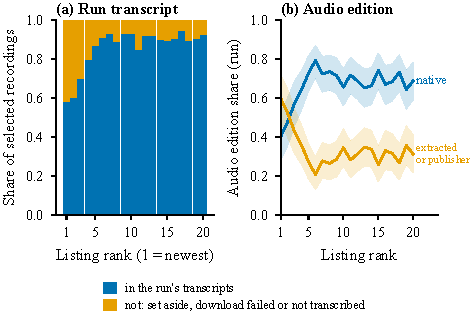
\includegraphics[width=\columnwidth]{floats/fig_rank.pdf}
\caption{Coverage of the newest-20 quota by listing rank (1 is the newest; listing order, not time): (a) share of the
\NSelected{} selected recordings with a run transcript and without one (set aside, download failed or not transcribed,
merged); (b) share of native platform audio among the recordings in the run, and of the other editions merged, with
95\% creator-bootstrap bands. A creator has at most one recording at a rank, so each cell is a count of creators, and
every cell holds 5 or more; the split by reason is in Table~\ref{tab:rank-odds}. Description of coverage; no trend is
read from rank.}
\label{fig:rank}
\end{figure}

\begin{table*}[tp]
\centering
\small
% tab_rank_odds.tex: GENERATED by the private builder build_numbers.py at 2026-11-26T03:59:48Z; label tab:rank-odds. The writer adds the float,
% the caption and the label. Sources: a private file of the run (named in the private build record)
% Creator-stratified Mantel-Haenszel and pooled ORs with 95% creator bootstrap; SMDs with 90% creator bootstrap. n.p.: the creators of 'no text of any kind' are not printed (D49).
{\scriptsize\setlength{\tabcolsep}{2pt}
\begin{tabular}{@{}p{0.36\textwidth}llll@{}}
\toprule
Outcome (ranks 1--5 against 6--20) & Pooled OR [95\%] & MH OR [95\%] & Cond.\ logit [95\% Wald] & Cr. \\
\midrule
not transcribed (any reason) & 4.12 [2.70, 6.95] & 5.47 [3.34, 9.75] & 7.15 [5.11, 10.0] & 84 \\
no text of any kind (download failed or not transcribed) & 1.04 [0.52, 1.92] & 1.04 [0.50, 1.95] & 1.04 [0.57, 1.89] & n.p. \\
other text kind or language review & 5.57 [3.28, 13.4] & 10.4 [4.97, 33.9] & 19.5 [11.8, 32.4] & 68 \\
\midrule
\multicolumn{5}{@{}p{0.97\linewidth}}{\emph{Transcribed (T) against other text (O) and missing (M): SMD [90\%]}} \\
log length (minutes; metadata, inventory or catalogue) & O: 0.12 [\ensuremath{-}0.03, 0.26] & M: \ensuremath{-}0.76 [\ensuremath{-}1.07, \ensuremath{-}0.44] &  &  \\
listing rank (1 = newest) & O: \ensuremath{-}0.76 [\ensuremath{-}1.14, \ensuremath{-}0.53] & M: \ensuremath{-}0.09 [\ensuremath{-}0.34, 0.13] &  &  \\
rank 1 to 5 (share) & O: 0.87 [0.62, 1.31] & M: 0.11 [\ensuremath{-}0.11, 0.36] &  &  \\
date evidence E1, confirmed day (share) & O: \ensuremath{-}0.61 [\ensuremath{-}0.95, \ensuremath{-}0.25] & M: 0.12 [\ensuremath{-}0.15, 0.39] &  &  \\
date evidence E3, still estimated (share) & O: 0.86 [0.49, 1.21] & M: \ensuremath{-}0.35 [\ensuremath{-}0.51, \ensuremath{-}0.14] &  &  \\
audio from the platform video (share of recordings with audio) & O: -- & M: 0.36 [0.24, 0.46] &  &  \\
publisher audio edition (share of recordings with audio) & O: -- & M: \ensuremath{-}0.36 [\ensuremath{-}0.46, \ensuremath{-}0.24] &  &  \\
log(1 + views at capture), seen creators only & O: 0.15 [\ensuremath{-}0.10, 0.42] & M: \ensuremath{-}0.14 [\ensuremath{-}0.45, 0.18] &  &  \\
\bottomrule
\end{tabular}}

\caption{Missingness by listing rank and recording properties. Top: odds ratios for ranks 1--5 against 6--20, pooled
(0.5 added per cell), Mantel--Haenszel within creator and conditional logit, with 95\% creator-bootstrap intervals, and
the creators with variation in the outcome. Bottom: standardized mean differences of recordings with other text (O) and
of recordings with no text (M) against transcribed recordings, with 90\% creator-bootstrap intervals. Event counts and
group sizes are not printed: beside the census counts some would give a cell of fewer than 5 by difference.}
\label{tab:rank-odds}
\end{table*}

\begin{figure}[ht]
\centering
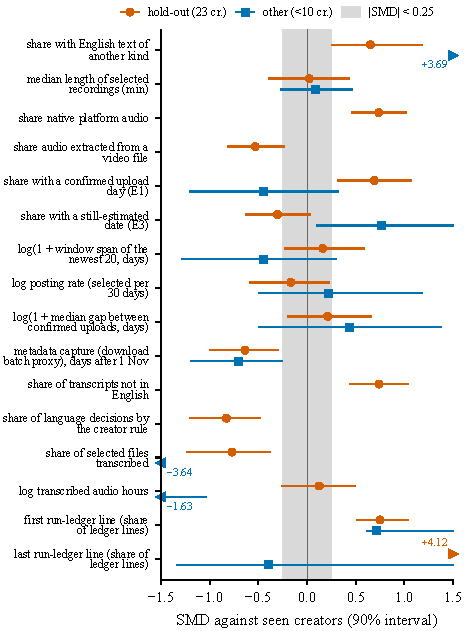
\includegraphics[width=\columnwidth]{floats/fig_love.pdf}
\caption{Standardized mean differences of creator values on ledger and inventory fields only: hold-out (\NHoldout)
minus seen (\NSeen) and other (\NOtherCreators) minus seen, with 90\% intervals from creator resamples within group,
clipped at $\pm$1 (values beyond the edge printed beside it); dashed lines $\pm$0.25, dotted $\pm$0.1. With
\NOtherCreators{} creators the other group's differences are unstable. The binary roster-vintage field is not drawn
(its signed differences would give group cells of fewer than 5 creators), and neither is a group's difference that
rests on fewer than 5 creators with a value other than the group's common one, nor a field where the seen group has
1 to 4 such creators. No transcript field of a non-seen creator was read.}
\label{fig:love}
\end{figure}

\begin{table*}[tp]
\centering
\small
% tab_balance.tex: GENERATED by the private builder build_numbers.py at 2026-11-26T03:59:48Z; label tab:balance. The writer adds the float,
% the caption and the label. Sources: a private file of the run (named in the private build record)
% Counts, durations, dates, languages and run order only (not contacts).
{\scriptsize\setlength{\tabcolsep}{2pt}
\begin{tabular}{@{}p{0.30\textwidth}clllll@{}}
\toprule
Covariate & Block & Seen: median (IQR) & Hold-out: median (IQR) & SMD hold-out [90\%] & SMD other [90\%] \\
\midrule
share with English text of another kind & A & 0.05 (0.00--0.10) & 0.10 (0.05--0.15) & 0.65 [0.26, 1.18] & 3.69 [3.16, 5.70] \\
median length of selected recordings (min) & A & 18.68 (11.01--28.79) & 15.85 (9.64--33.38) & 0.02 [\ensuremath{-}0.39, 0.43] & 0.08 [\ensuremath{-}0.27, 0.46] \\
share native platform audio & A & 0.76 (0.42--0.89) & 0.84 (0.78--0.90) & 0.74 [0.46, 1.02] & -- \\
share audio extracted from a video file & A & 0.20 (0.09--0.46) & 0.16 (0.10--0.20) & \ensuremath{-}0.53 [\ensuremath{-}0.81, \ensuremath{-}0.24] & -- \\
share with a confirmed upload day (E1) & A & 0.90 (0.70--0.95) & 0.95 (0.90--1.00) & 0.69 [0.32, 1.07] & \ensuremath{-}0.45 [\ensuremath{-}1.20, 0.31] \\
share with a still-estimated date (E3) & A & 0.05 (0.00--0.10) & 0.05 (0.00--0.10) & \ensuremath{-}0.30 [\ensuremath{-}0.62, 0.03] & 0.77 [0.10, 1.59] \\
log(1 + window span of the newest 20, days) & A & 5.04 (4.52--6.27) & 5.67 (4.91--5.97) & 0.16 [\ensuremath{-}0.23, 0.58] & \ensuremath{-}0.45 [\ensuremath{-}1.28, 0.29] \\
log posting rate (selected per 30 days) & A & 1.36 (0.13--1.89) & 0.73 (0.43--1.49) & \ensuremath{-}0.17 [\ensuremath{-}0.58, 0.22] & 0.22 [\ensuremath{-}0.49, 1.18] \\
log(1 + median gap between confirmed uploads, days) & A & 2.08 (1.50--2.30) & 2.08 (1.79--2.74) & 0.21 [\ensuremath{-}0.20, 0.66] & 0.43 [\ensuremath{-}0.49, 1.37] \\
metadata capture (download batch proxy), days after 1 Nov & A & 17.75 (17.34--18.93) & 17.75 (17.34--17.77) & \ensuremath{-}0.64 [\ensuremath{-}0.99, \ensuremath{-}0.30] & \ensuremath{-}0.71 [\ensuremath{-}1.19, \ensuremath{-}0.26] \\
share of transcripts not in English & L & 0.00 (0.00--0.00) & 0.00 (--) & 0.74 [0.44, 1.03] & -- \\
share of language decisions by the creator rule & L & 0.84 (0.80--0.88) & 0.83 (0.27--0.88) & \ensuremath{-}0.83 [\ensuremath{-}1.20, \ensuremath{-}0.48] & -- \\
share of selected files transcribed & R & 0.90 (0.90--0.95) & 0.85 (0.80--0.91) & \ensuremath{-}0.77 [\ensuremath{-}1.23, \ensuremath{-}0.38] & \ensuremath{-}3.64 [\ensuremath{-}5.64, \ensuremath{-}3.07] \\
log transcribed audio hours & R & 1.94 (1.41--2.38) & 1.99 (1.51--2.36) & 0.13 [\ensuremath{-}0.26, 0.49] & \ensuremath{-}1.63 [\ensuremath{-}2.92, \ensuremath{-}1.04] \\
first run-ledger line (share of the run's ledger lines) & Q & 0.03 (0.01--0.04) & 0.08 (0.03--0.12) & 0.75 [0.51, 1.04] & 0.71 [0.62, 1.61] \\
last run-ledger line (share of the run's ledger lines) & Q & 0.76 (0.75--0.77) & 0.95 (0.95--0.96) & 4.12 [2.92, 10.48] & \ensuremath{-}0.40 [\ensuremath{-}1.33, 2.55] \\
\midrule
\multicolumn{6}{@{}p{0.97\linewidth}}{\emph{Roster vintage, all creators: 74 original, 27 added on the day of the listing}} \\
\multicolumn{6}{@{}p{0.97\linewidth}}{\emph{Hold-out membership AUC: A 0.69 (shuffle 95\% band 0.30--0.67); A + language decisions 0.84 (shuffle 95\% band 0.32--0.66)}} \\
\bottomrule
\end{tabular}}

\caption{Table B: balance of the seen, hold-out and other creators on fields known before the run, with medians and
quartiles for the seen and hold-out groups (with \NOtherCreators{} creators the other group's median would be a
single value of the group, so only its standardized mean difference is printed; ``--'' marks hold-out quartiles that
would interpolate a single value)
and standardized mean differences (90\% creator-bootstrap intervals; ``--'' where the group's difference rests on fewer
than 5 creators with a value other than the group's common one, and a field left out where the seen group has 1 to 4
such creators); the roster vintage of all creators only (by group,
and as a signed difference of a binary field, it would give cells of fewer than 5 creators); and the cross-validated AUC of hold-out membership on \DTwoFields{} pre-run fields, \DTwoAuc{} against a
999-shuffle 95\% band of \DTwoAucBandLo--\DTwoAucBandHi.}
\label{tab:balance}
\end{table*}

\paragraph{Time without speech.} Moved here from Section 4 by the page limit (fourth review round): the voice
detector's non-speech is recomputed as audio minus detector speech seconds, because the stored field is zero in some
transcripts; time outside recognizer segments is a second definition. No independent voice detector, forced aligner or
speaker separation (no new audio-analysis packages, registry 02:50) and no re-probe of creator-rule files was run.
Figure~\ref{fig:coverage} shows coverage by recognizer segments by position,
Figure~\ref{fig:classes} splits running time into classes by position, and Table~\ref{tab:nonspeech} gives both
definitions of time without speech under three weightings (Section~\ref{sec:nonspeech}). Moved here from Section 5.5
by the page limit: the voice detector's non-speech is \NonSpeechMedianPct\% at the creator median; \OutsideSegEdgesPct{}
points of the time outside recognizer segments (\OutsideSegPooledPct\%, 95\% \OutsideSegPooledLo--\OutsideSegPooledHi)
lie before the first or after the last segment, and long pauses count as non-speech. The last 15\,s are covered
\LastFifteenCoverage, the 15\,s before them \FifteenToThirtyCoverage{} and the first 15\,s \FirstFifteenCoverage. The
last 60\,s hold about \LastSixtyRatio{} times the share outside recognized speech of the rest (\LastSixtyOutsidePct\%
against \RestOutsidePct\%, hours pooled; Figure~\ref{fig:classes}). Across weightings and windows, the non-speech
headline leaves its pre-set margin in \RFourNonspeechMoves{} of \RFourSpecs{} specifications and end coverage in
\RFourEndCoverageMoves{} (Figure~\ref{fig:sensitivity}). The share of transcripts with a thanks segment anywhere is
\ThanksAnywherePct\% by GRID's definition (Table~\ref{tab:headlines} gives D4's).

% Moved here from Section 5.5 by the page limit (third review round); caption unchanged.
\begin{figure}[ht]
\centering
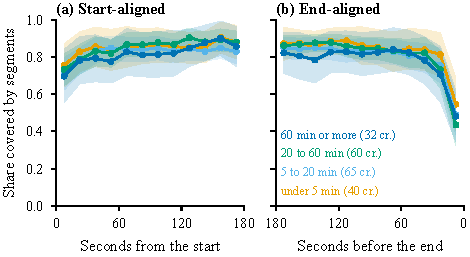
\includegraphics[width=\columnwidth]{floats/fig_coverage.pdf}
\caption{Share of each 15-s bin inside recognizer segments (filter version 2), aligned at the start (top) and at the
end (bottom) of the recording, by length band, \NSeen{} seen creators weighted equally. Grey: sup-$t$ simultaneous 95\%
band from creator-then-recording resamples; dotted: pointwise 95\%; dashed: all lengths; axis 0 to 1; bins under 5
creators omitted. Seen creators only: no positional display of the hold-out is drawn.}
\label{fig:coverage}
\end{figure}

\begin{figure}[ht]
\centering
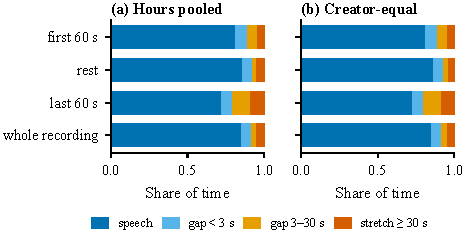
\includegraphics[width=\columnwidth]{floats/fig_classes.pdf}
\caption{Running time inside recognizer segments, in gaps under 3\,s, in gaps of 3--30\,s and in stretches of 30\,s or
more (filter version 2), for the whole recording, the first 60\,s, the rest and the last 60\,s; (a) hours pooled, (b)
creators weighted equally, with 95\% creator-bootstrap intervals; \NSeen{} seen creators. Music, meditation and silence
cannot be told apart.}
\label{fig:classes}
\end{figure}

\begin{table*}[tp]
\centering
\small
% tab_nonspeech.tex: GENERATED by the private builder build_numbers.py at 2026-11-26T03:59:48Z; label tab:nonspeech. The writer adds the float,
% the caption and the label. Sources: a private file of the run (named in the private build record)
% Seen creators; percentages of audio time.
{\scriptsize\setlength{\tabcolsep}{2pt}
\begin{tabular}{@{}p{0.34\textwidth}rlll@{}}
\toprule
Definition & Hours & Pooled \% [95\%] & Creator-equal \% [$t$ 95\%] & Creator median \% [95\%] \\
\midrule
voice detector's non-speech (audio minus detector speech seconds) & 66.4 & 12.1 [7.7, 17.5] & 12.2 [8.7, 15.6] & 7.9 [5.3, 10.9] \\
time outside recognizer segments, artefact filter v2 & 81.3 & 14.8 [10.9, 19.9] & 14.9 [11.8, 18.0] & 11.4 [9.6, 12.9] \\
time outside recognizer segments, no filter & 81.1 & 14.8 [10.9, 19.9] & 14.9 [11.8, 17.9] & 11.4 [9.5, 12.9] \\
of which before the first or after the last segment (filter v2) & 24.4 & 4.4 [1.2, 9.8] & 3.8 [1.2, 6.4] & 0.8 [0.5, 1.3] \\
\midrule
\multicolumn{5}{@{}p{0.97\linewidth}}{\emph{Coverage by recognizer segments (filter v2), creator-equal [95\%]}} \\
last partial decoding window (creator-equal) &  & 0.48 [0.41, 0.54] & 71 cr. & 1{,}208 rec. \\
full 30-s window before it (creator-equal) &  & 0.78 [0.73, 0.82] & 71 cr. & 1{,}208 rec. \\
difference, last partial minus window before &  & \ensuremath{-}0.30 [\ensuremath{-}0.35, \ensuremath{-}0.26] & 71 cr. & 1{,}208 rec. \\
middle: 180 s from the start to 180 s before the end, recordings of 6 min or more (creator-equal) &  & 0.87 [0.85, 0.90] & all but $<$5 cr. & 1{,}053 rec. \\
last 15 s (all lengths) &  & 0.49 [0.42, 0.55] & 71 cr. & 1{,}293 rec. \\
15 to 30 s before the end (all lengths) &  & 0.77 [0.71, 0.82] & 71 cr. & 1{,}293 rec. \\
first 15 s (all lengths) &  & 0.75 [0.70, 0.80] & 71 cr. & 1{,}293 rec. \\
\midrule
\multicolumn{5}{@{}p{0.97\linewidth}}{Segment-gap share minus detector share per recording: median 3.5 points (P10 -2.4, P90 6.9); Spearman 0.89} \\
\bottomrule
\end{tabular}}

\caption{Share of audio without speech, seen creators: the voice detector's non-speech and time outside recognizer
segments (filter version 2 and none), pooled over hours, creator-equal and at the creator median, with 95\% intervals and
leave-one-creator-out ranges; and the coverage of the last partial decoding window against the window before it.}
\label{tab:nonspeech}
\end{table*}

\paragraph{Variance and error tolerance.} Moved here from Section 5.7 by the page limit (results round): the caption
anchor's creator mean has a 95\% $t$ bound up to \AnchorCaptionMeanTHi\% and is \AnchorCaptionPooledPct\% pooled, so the
tolerance thresholds lie near either form of the measured machine disagreement; error that differs between creators
can link word length, MATTR-1000 and filled pauses to the share without speech, so their between-creator comparisons
carry a caveat. Figure~\ref{fig:icc} shows the share of variance between creators for each
measure, and Table~\ref{tab:vp} is the full variance partition behind it; Figure~\ref{fig:tolerance} and
Table~\ref{tab:tolerance} give the error tolerance of the word measures (Section~\ref{sec:variance}). Tolerance is not
accuracy. Moved here from Section 5.7 by the page limit: error that differs between creators and tracks non-speech can
move their creator-level correlation with non-speech share by up to \RSixAssocMax{} either way (word length, MATTR-1000)
and \RSixFillerAssoc{} (filled pauses) at a 10\% median; pronoun, contraction, question-mark and numeral rates, pace and
log words keep their structure. Every between-creator comparison of word length, MATTR or filled-pause rate carries this
caveat. The MATTR window is 500 words for the ICC, 1,000 in the tolerance and 100 in the bridge (``variety'').
Gaussian and logit ICC intervals rest on \VpDrawsGauss{} creator draws. Moved here from Section 5.7 by the page limit
(fourth review round): the ANOVA estimate of the earlier draft for mean segment log-probability is \IccSegLogpAnova{}
(\IccSegLogpAnovaLo--\IccSegLogpAnovaHi); negative-binomial intervals rest on \VpDrawsNb{} creator draws; parametric
intervals are \ParamNarrowLo{} to \ParamNarrowHi{} times narrower for \ParamNarrowRows{} of the \VpMeasures{} measures;
for first-person singular the point values are \IccFsRaw{} (raw) and \IccFsLog{} (log), an illustration of scale, and
\IccFs{} on the latent scale (95\% \IccFsLo--\IccFsHi).

% INTEGRATOR: moved here from Section 5.7 by the P7 move log (build of 2026-11-21 07:05 UTC); caption unchanged.
\begin{figure}[tp]
\centering
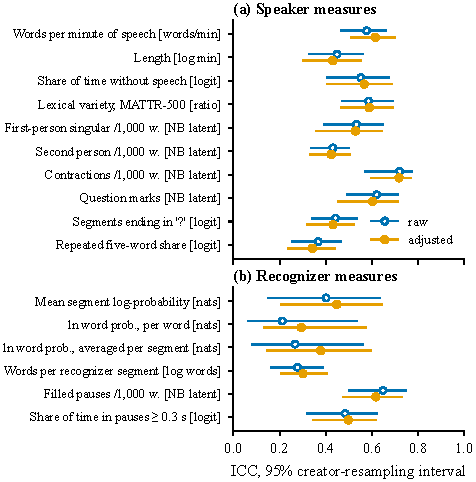
\includegraphics[width=\columnwidth]{floats/fig_icc.pdf}
\caption{Share of variance between creators (ICC) for word and timing measures (a) and recognizer measures (b), on
\VpCreators{} seen creators and \VpRecordings{} recordings (filter version 2), each on the scale named in its label: raw
(open) and adjusted for log length, edition and median word probability (filled), with 95\% creator-resampling
intervals; grey bars: parametric intervals, for comparison only. A design fact of this roster.}
\label{fig:icc}
\end{figure}

\begin{table*}[tp]
\centering
\small
% tab_vp.tex: GENERATED by WORK/build_numbers.py at 2026-11-22T01:51:42Z; label tab:vp. The writer adds the float,
% the caption and the label. Sources: REV/build-robustness/out/R5/R5-VP1-variance-partition.csv
% CB: creator-resampling bootstrap; CB/PB: width of the creator bootstrap over the parametric interval.
{\scriptsize\setlength{\tabcolsep}{2.5pt}
\begin{tabular}{@{}p{0.2\textwidth}p{0.11\textwidth}llrlrrrr@{}}
\toprule
Measure & Scale & Panel & ICC raw [95\% CB] & CB/PB & Adjusted [95\% CB] & Filter off & Kish deff & $n_{\mathrm{eff}}$ & $R_{10}$ \\
\midrule
Words per minute of speech & identity (words/min) & speaker & 0.58 [0.47, 0.66] & 1.1 & 0.62 [0.51, 0.70] & 0.59 & 10.6 & 114 & 0.93 \\
Length & log minutes & speaker & 0.45 [0.33, 0.56] & 1.3 & 0.43 [0.30, 0.55] & 0.45 & 8.5 & 143 & 0.89 \\
Share of time without speech & logit of share & speaker & 0.55 [0.41, 0.67] & 1.5 & 0.57 [0.41, 0.68] & 0.55 & 10.2 & 119 & 0.93 \\
Lexical variety & identity (ratio) & speaker & 0.59 [0.47, 0.69] & 1.2 & 0.59 [0.47, 0.69] & 0.58 & 10.3 & 107 & 0.93 \\
First-person singular per 1,000 words & NB latent log-rate & speaker & 0.53 [0.40, 0.65] & 1.4 & 0.53 [0.36, 0.64] & 0.53 & 9.9 & 123 & 0.92 \\
Second person per 1,000 words & NB latent log-rate & speaker & 0.43 [0.34, 0.50] & 0.9 & 0.42 [0.33, 0.50] & 0.43 & 8.2 & 148 & 0.88 \\
Contractions per 1,000 words & NB latent log-rate & speaker & 0.72 [0.57, 0.77] & 1.3 & 0.72 [0.60, 0.77] & 0.72 & 13.0 & 93 & 0.96 \\
Question marks per 1,000 words & NB latent log-rate & speaker & 0.62 [0.49, 0.71] & 1.2 & 0.60 [0.46, 0.71] & 0.62 & 11.3 & 107 & 0.94 \\
Segments ending in '?' & logit of share & speaker & 0.44 [0.34, 0.53] & 1.1 & 0.43 [0.32, 0.52] & 0.44 & 8.4 & 145 & 0.89 \\
Repeated five-word share & logit of share & speaker & 0.37 [0.26, 0.46] & 1.2 & 0.34 [0.24, 0.44] & 0.37 & 7.1 & 170 & 0.85 \\
Mean segment log-probability & identity (nats) & recognizer & 0.40 [0.15, 0.63] & 2.7 & 0.45 [0.21, 0.64] & 0.40 & 7.7 & 157 & 0.87 \\
Mean ln word probability, per word & identity (nats) & recognizer & 0.21 [0.06, 0.53] & 3.6 & 0.29 [0.13, 0.57] & 0.22 & 4.5 & 268 & 0.73 \\
Mean ln word probability, averaged per segment & identity (nats) & recognizer & 0.27 [0.08, 0.56] & 3.0 & 0.38 [0.15, 0.59] & 0.27 & 5.5 & 222 & 0.79 \\
Words per recognizer segment & log words & recognizer & 0.28 [0.16, 0.39] & 1.4 & 0.30 [0.21, 0.40] & 0.28 & 5.6 & 215 & 0.79 \\
Filled pauses per 1,000 words & NB latent log-rate & recognizer & 0.65 [0.50, 0.75] & 1.2 & 0.62 [0.47, 0.73] & 0.65 & 11.8 & 103 & 0.95 \\
Share of time in pauses $\geq$ 0.3 s & logit of share & recognizer & 0.48 [0.32, 0.62] & 1.6 & 0.50 [0.35, 0.62] & 0.47 & 9.1 & 133 & 0.90 \\
\bottomrule
\end{tabular}}

\caption{Table VP-1, condensed: measure, scale, raw ICC with its 95\% creator-resampling interval, adjusted ICC (log
length, edition, median word probability), ICC with the filter off, Kish design effect, effective recordings and the
reliability of a ten-recording creator mean; \VpCreators{} seen creators, \VpRecordings{} recordings, filter version 2.
The ICC is a design fact of this roster.}
\label{tab:vp}
\end{table*}

\begin{figure*}[tp]
\centering
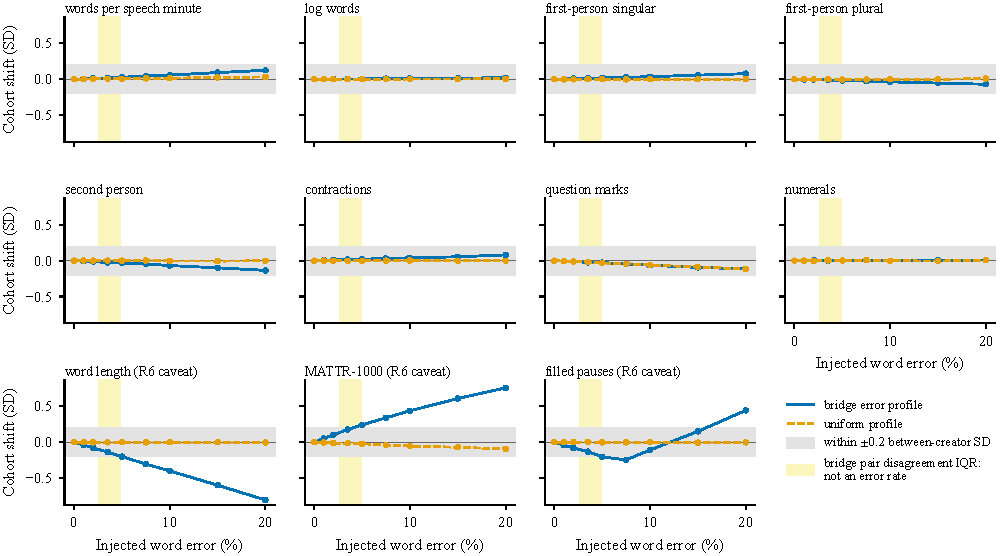
\includegraphics[width=\textwidth]{floats/fig_tolerance.pdf}
\caption{Injected word error (0--20\%) against each word measure's creator-equal cohort mean relative to its clean
value, with the bridge's edit profile (solid) and a uniform profile (dashed); grey: 10th--90th percentile over creators;
dotted: $\pm$0.2 between-creator SD. The vertical band marks the bridge's model-to-model disagreement, which is not an
error rate. Tolerance, not accuracy.}
\label{fig:tolerance}
\end{figure*}

\begin{table}[ht]
\centering
\small
% tab_tolerance.tex: GENERATED by WORK/build_numbers.py at 2026-11-22T01:51:42Z; label tab:tolerance. The writer adds the float,
% the caption and the label. Sources: REV/build-robustness/out/R6/R6-tolerance-table.csv; REV/build-robustness/out/R6/R6-creator-error-scenarios.csv
% First three columns: injected error (per cent, bridge profile, same rate for every creator) at which the cohort mean, the median creator and the 90th-percentile creator move 0.2 between-creator SD. Last three: creator-differing error (sigma 0.86, rho 0.7 with non-speech share) at a 3.5% median: Spearman of creator means with the clean ones, and change of the creator-level correlation with non-speech share at 3.5% and 10% medians.
{\scriptsize\setlength{\tabcolsep}{2pt}
\begin{tabular}{@{}p{0.2\linewidth}rrrrrrrr@{}}
\toprule
Measure & Coh. & Med. & P90 & 3.5\% & ICC$_{20}$ & $\rho$ & $\Delta\rho_{3.5}$ & $\Delta\rho_{10}$ \\
\midrule
log words & $>$20 & $>$20 & $>$20 & 0.00 & 0.45 & 1.00 & 0.00 & 0.01 \\
words per speech minute & $>$20 & $>$20 & $>$20 & 0.02 & 0.58 & 1.00 & 0.02 & 0.04 \\
mean word length (letters) & 5.0 & 5.2 & 3.8 & \ensuremath{-}0.14 & 0.57 & 0.92 & \ensuremath{-}0.16 & \ensuremath{-}0.27 \\
MATTR (1,000) & 4.0 & 4.2 & 3.2 & 0.18 & 0.64 & 0.91 & 0.18 & 0.26 \\
contractions /1,000 & $>$20 & $>$20 & 14.1 & 0.02 & 0.60 & 1.00 & 0.03 & 0.05 \\
first-person singular /1,000 & $>$20 & $>$20 & 13.4 & 0.01 & 0.28 & 1.00 & 0.00 & 0.02 \\
first-person plural /1,000 & $>$20 & $>$20 & 19.9 & \ensuremath{-}0.01 & 0.37 & 1.00 & 0.00 & 0.00 \\
second person /1,000 & $>$20 & $>$20 & 14.6 & \ensuremath{-}0.03 & 0.43 & 1.00 & \ensuremath{-}0.02 & \ensuremath{-}0.04 \\
question marks /1,000 & $>$20 & $>$20 & 17.8 & \ensuremath{-}0.02 & 0.30 & 1.00 & 0.00 & \ensuremath{-}0.01 \\
filled pauses /1,000 & 4.9 & 4.7 & 1.1 & \ensuremath{-}0.13 & 0.01 & 0.71 & 0.18 & 0.43 \\
numerals /1,000 & $>$20 & $>$20 & $>$20 & 0.00 & 0.25 & 1.00 & 0.01 & 0.01 \\
\bottomrule
\end{tabular}}

\caption{Injected error rate at which the cohort mean, the median creator and the 90th-percentile creator move by 0.2
between-creator SD, by edit profile, with the same rate for every creator; and the scenarios in which the error rate
differs between creators and tracks pace or the share of time without speech. ICC$_{20}$ is the ICC at 20\% injected
error, a simulation summary without interval. Between-creator comparisons of word length, MATTR and filled-pause rate
carry the caveat of Section~\ref{sec:variance}.}
\label{tab:tolerance}
\end{table}

\paragraph{Bridge.} Table~\ref{tab:bridge-verdicts} gives the bridge verdicts under both scales and both kinds of
interval (Section~\ref{sec:bridge}). The figure of mean paired differences and the Bland--Altman summaries of earlier
drafts are not printed (fourth review round): beside the registered bridge results, the seen pairs' means, intervals
and limits of agreement would give single pairs' values by difference, and a bin median of a fifth of the pairs is one
pair's value.

\begin{table}[ht]
\centering
\small
% tab_bridge_verdicts.tex: GENERATED by WORK/build_numbers.py at 2026-11-22T01:51:42Z; label tab:bridge-verdicts. The writer adds the float,
% the caption and the label. Sources: REV/build-robustness/out/R3/R3-bridge-verdicts.csv
% The seen pairs (all but fewer than 5 of the registered pairs, one per creator; their count is not printed); margin +/-0.2 SD; verdicts only (round 4: no seen-pair mean, interval or limit of agreement, no drop column). Each verdict equals the verdict on all registered pairs; no single-pair drop moves a verdict between agrees and differs.
{\scriptsize\setlength{\tabcolsep}{3pt}
\begin{tabular}{@{}p{0.40\linewidth}llll@{}}
\toprule
Measure & Between & Betw.\ sim. & Within & With.\ sim. \\
\midrule
Contracted forms /1,000 & agrees & agrees & agrees & agrees \\
Distinct words in 100-word windows & agrees & agrees & agrees & agrees \\
First-person plural /1,000 & agrees & agrees & agrees & agrees \\
First-person singular /1,000 & agrees & agrees & agrees & agrees \\
Mean word length (letters) & agrees & agrees & agrees & open \\
Second person /1,000 & agrees & agrees & agrees & agrees \\
Words per minute of speech & agrees & agrees & agrees & agrees \\
Isolated short segments, per hour & open & open & open & open \\
Loop words removed /1,000 & open & open & agrees & agrees \\
Mean word probability & open & open & open & open \\
Thanks phrase removed, per hour & open & open & open & open \\
Filled pauses /1,000 & differs & differs & differs & differs \\
Mean word duration (s) & differs & differs & differs & differs \\
Pauses 0.3-1 s per speech minute & differs & differs & differs & differs \\
Pauses $\geq$ 1 s per speech minute & differs & differs & differs & differs \\
Share of time in pauses $\geq$ 0.3 s & differs & differs & differs & differs \\
Words per recognizer segment & differs & differs & differs & open \\
\bottomrule
\end{tabular}}

\caption{Bridge verdicts per measure on the between-creator (Between) and the within-creator scale (Within), with
per-measure and simultaneous (sim.) 90\% $t$ intervals against the margin of $\pm$\BridgeMargin{} SD fixed in advance, on \BridgeSeenPairs{} seen pairs
(all but fewer than 5 of its \BridgePairs{} registered pairs); verdicts only, each equal to the verdict on all registered pairs. No single-pair drop moves a verdict between agrees and differs. The verdicts concern means over English
audio of 5--60 minutes, not single recordings or other languages; neither transcript is a human reference.}
\label{tab:bridge-verdicts}
\end{table}

\paragraph{Weighting and window sensitivity.} Figure~\ref{fig:sensitivity} and Table~\ref{tab:sensitivity} show each
headline under other weightings and windows, against a margin fixed before the run.

\begin{figure*}[tp]
\centering
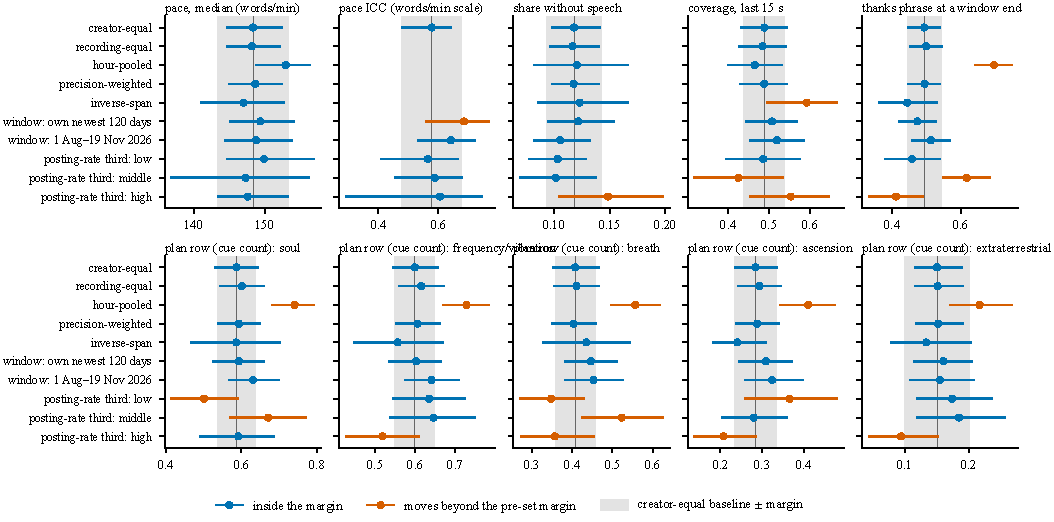
\includegraphics[width=\textwidth]{floats/fig_sensitivity.pdf}
\caption{Headline numbers, and the reporting plan's cue-count robustness rows (``plan row''), under five weightings and
three restrictions (each creator's own newest 120 days, a fixed calendar window, thirds of posting rate), with
creator-bootstrap 90\% intervals; grey band: the creator-equal baseline $\pm$ the margin fixed before the run. In this
roster, under the newest-20 quota; no period or trend.}
\label{fig:sensitivity}
\end{figure*}

\begin{table*}[tp]
\centering
\small
% tab_sensitivity.tex: GENERATED by WORK/build_numbers.py at 2026-11-22T00:15:32Z; label tab:sensitivity. The writer adds the float,
% the caption and the label. Sources: REV/build-robustness/out/R4/R4-summary-table.csv
{\scriptsize\setlength{\tabcolsep}{2.5pt}
\begin{tabular}{@{}p{0.2\textwidth}rrlllp{0.33\textwidth}@{}}
\toprule
Headline & Baseline & Margin & Range & Beyond margin & Interval outside & Largest mover \\
\midrule
pace, median (words/min) & 148.4 & 5.0 & 146.6--153.6 & 2 of 40 & 0 & hour-pooled / own newest 120 days / none / all \\
pace, ICC & 0.578 & 0.100 & 0.565--0.685 & 1 of 6 & 0 & creator-equal / own newest 120 days / none / all \\
share without speech & 0.118 & 0.025 & 0.102--0.148 & 3 of 40 & 0 & creator-equal / all / none / high \\
speech coverage, last 15 s & 0.489 & 0.050 & 0.425--0.604 & 9 of 40 & 0 & inverse-span / calendar 2026-08-01 to 2026-11-19 / none / all \\
thanks phrase at a window end & 0.494 & 0.050 & 0.411--0.705 & 20 of 40 & 8 & hour-pooled / all / 5 min / all \\
robustness row of the plan (cue count, not a headline): cue share: soul & 0.587 & 0.050 & 0.501--0.784 & 19 of 40 & 7 & hour-pooled / calendar 2026-08-01 to 2026-11-19 / 5 min / all \\
robustness row of the plan (cue count, not a headline): cue share: frequency/vibration & 0.599 & 0.050 & 0.518--0.734 & 14 of 40 & 5 & hour-pooled / all / 5 min / all \\
robustness row of the plan (cue count, not a headline): cue share: breath & 0.408 & 0.050 & 0.348--0.576 & 15 of 40 & 7 & hour-pooled / own newest 120 days / 5 min / all \\
robustness row of the plan (cue count, not a headline): cue share: ascension & 0.285 & 0.050 & 0.208--0.415 & 9 of 40 & 3 & hour-pooled / all / 5 min / all \\
robustness row of the plan (cue count, not a headline): cue share: extraterrestrial/alien & 0.150 & 0.050 & 0.094--0.219 & 6 of 40 & 0 & hour-pooled / all / 5 min / all \\
\bottomrule
\end{tabular}}

\caption{Per headline: creator-equal baseline, the margin fixed before the run, the range over the \RFourSpecs{}
specifications, and how many move the estimate beyond the margin. Baselines are the sensitivity build's own
creator-equal estimates and can differ in the last digit from the figures of Section~\ref{sec:measure}. The term rows
are robustness rows of the reporting plan (cue counts), not headlines of this paper and not findings about channelling.}
\label{tab:sensitivity}
\end{table*}

\paragraph{Model-coded checks of the measurement.} Table~\ref{tab:kinds} is the interim census of recording kinds
(Section~\ref{sec:data}), Table~\ref{tab:nonlanguage} the pseudo-word flag (Section~\ref{sec:pipeline}) and
Table~\ref{tab:labelflips} how much the choice of recognizer moves model-coded labels. All three are model-coded and not
checked by a person.

\begin{table}[ht]
\centering
\small
% tab_kinds.tex: GENERATED by the private builder build_numbers.py at 2026-11-26T03:59:48Z; label tab:kinds. The writer adds the float,
% the caption and the label. Sources: a private file of the run (named in the private build record)
% Interim, model-coded, not checked by a person; development creators only; creator-weighted. Every kind and band holds 5 or more creators (checked with small_cells.pool_small_groups).
{\scriptsize\setlength{\tabcolsep}{2pt}
\begin{tabular}{@{}p{0.3\linewidth}llllr@{}}
\toprule
Kind (largest by words) & $n$ (S / M) & Rec.\ S \% [95\%] & Rec.\ M \% [95\%] & Agr. & Stab. \\
\midrule
Channelled (embodied) voice & 25 / 28 & 26 [17, 37] & 29 [20, 39] & 0.79 & 0.98 \\
Relayed message & 11 / 7 & 12 [4, 21] & 7 [2, 15] & 0.78 & 0.96 \\
Interview or podcast & 14 / 13 & 15 [7, 23] & 14 [6, 22] & 0.81 & 0.99 \\
Guided practice & 10 / 11 & 10 [4, 18] & 11 [5, 19] & 0.95 & 1.00 \\
Own-voice talk & 31 / 32 & 32 [22, 43] & 33 [24, 43] & 0.89 & 0.95 \\
Advert or other & 5 / 5 & 5 [1, 9] & 5 [1, 10] & 0.80 & 0.96 \\
\midrule
Main kind channelled or relayed & 36 / 35 & 38 [26, 49] & 37 [26, 47] & 0.85 & -- \\
\midrule
Claimed voice in any part & 70 / 59 & 73 [63, 84] & 62 [50, 73] & 0.90 & 0.91 \\
Claimed voice in 10\%+ of words & 50 / 48 & 52 [41, 64] & 50 [38, 62] & 0.88 & 0.93 \\
Claimed voice in 25\%+ of words & 43 / 40 & 45 [34, 56] & 42 [31, 52] & 0.87 & 0.94 \\
\midrule
\multicolumn{6}{@{}p{0.97\linewidth}}{\emph{Claimed-voice band of a recording, creator-weighted \% [95\%], small / middle}} \\
0 & 26 / 37 & 27 [16, 37] & 38 [27, 50] &  &  \\
under 10 & 20 / 11 & 21 [13, 30] & 12 [4, 20] &  &  \\
10 to 25 & 7 / 8 & 7 [2, 13] & 8 [2, 16] &  &  \\
25 to 50 & 12 / 10 & 13 [6, 20] & 11 [4, 18] &  &  \\
50 or more & 31 / 30 & 32 [22, 43] & 31 [22, 42] &  &  \\
\bottomrule
\end{tabular}}

\caption{Interim census of recording kinds and claimed-voice bands on \LOneRecordings{} recordings of \LOneCreators{}
development creators: creator-weighted shares of recordings and of speech hours with 95\% creator-bootstrap intervals,
under the small model (modal kind of five runs) and the middle model, with their specific agreement and run-to-run
stability. Model-coded, not checked by a person; development creators only; interim. It replaces the earlier draft's
count from a purposive reading.}
\label{tab:kinds}
\end{table}

\begin{table}[ht]
\centering
\small
% tab_nonlanguage.tex: GENERATED by the private builder build_numbers.py at 2026-11-26T03:59:48Z; label tab:nonlanguage. The writer adds the float,
% the caption and the label. Sources: a private file of the run (named in the private build record)
% Model-read (both model tiers agree), not checked by a person; window level with creator bootstrap. Lower block: with / without flagged windows.
{\scriptsize\setlength{\tabcolsep}{2pt}
\begin{tabular}{@{}p{0.11\linewidth}p{0.17\linewidth}rrp{0.16\linewidth}p{0.16\linewidth}@{}}
\toprule
Sample & Creators & Windows & Cr. & Coherent language [95\%] & Non-language [95\%] \\
\midrule
flagged & all seen & 200 & 56 & 0.38\newline[0.24, 0.67] & 0.51\newline[0.19, 0.68] \\
flagged & development & 147 & 42 & 0.52\newline[0.31, 0.79] & 0.36\newline[0.08, 0.61] \\
flagged & check & 53 & 14 & 0.21\newline[0.10, 0.77] & 0.70\newline[0.19, 0.88] \\
unflagged & all seen & 200 & 71 & 1.00\newline[1.00, 1.00] & 0.00\newline[0.00, 0.00] \\
unflagged & development & 135 & 48 & 1.00\newline[1.00, 1.00] & 0.00\newline[0.00, 0.00] \\
unflagged & check & 65 & 23 & 1.00\newline[1.00, 1.00] & 0.00\newline[0.00, 0.00] \\
\midrule
\multicolumn{6}{@{}p{0.97\linewidth}}{\emph{Lexical measures with and without flagged windows (creator means [95\%])}} \\
MATTR &  &  & 71 & 0.647\newline[0.640, 0.655] & 0.647\newline[0.640, 0.655] \\
types per 1,000 words &  &  & all but $<$5 & 338.8\newline[330.6, 347.1] & 338.4\newline[330.1, 346.5] \\
words per minute &  &  & 71 & 148.6\newline[144.7, 152.4] & 148.9\newline[145.0, 152.8] \\
names per 1,000 words &  &  & 71 & 2.749\newline[2.175, 3.403] & 2.744\newline[2.170, 3.393] \\
\bottomrule
\end{tabular}}

\caption{Pseudo-word flag, fixed on development creators before any reading: model-read share of flagged and unflagged
30-s windows read as non-language, weighted to all windows of each stratum, and lexical measures with and without the
flagged windows. Model-read: without audio a reader cannot tell glossolalia from misrecognised speech or another
language.}
\label{tab:nonlanguage}
\end{table}

\begin{table}[ht]
\centering
\small
% tab_labelflips.tex: GENERATED by WORK/build_numbers.py at 2026-11-22T00:15:32Z; label tab:labelflips. The writer adds the float,
% the caption and the label. Sources: REV/build-llm/out/L2/tab-L2-label-flips.csv; REV/build-llm/out/L2/L2-summary.json
% Model-coded; rows the L2 build marks as shown (enough recordings). Rec.: bridge recordings of development creators, one per creator; a count fewer than 5 below a count it is nested in is printed as 'all but <5'.
{\scriptsize\setlength{\tabcolsep}{2pt}
\begin{tabular}{@{}lp{0.24\linewidth}lrp{0.14\linewidth}p{0.14\linewidth}p{0.14\linewidth}@{}}
\toprule
Instr. & Label & Unit & Rec. & Between transcripts [90\%] & Run to run [90\%] & Difference [90\%] \\
\midrule
voice & all labels (share of words) & words & 25 & 0.19\newline[0.10, 0.28] & 0.22\newline[0.13, 0.31] & \ensuremath{-}0.02\newline[\ensuremath{-}0.08, 0.02] \\
voice & claimed voice (V2 or V3) (1 - Jaccard) & words & 16 & 0.21\newline[0.11, 0.36] & 0.27\newline[0.13, 0.48] & \ensuremath{-}0.06\newline[\ensuremath{-}0.14, 0.02] \\
voice & claimed or not (share of all words) & words & 16 & 0.07\newline[0.04, 0.11] & 0.09\newline[0.04, 0.15] & \ensuremath{-}0.02\newline[\ensuremath{-}0.06, 0.01] \\
voice & V1 own person (1 - Jaccard) & words & all but $<$5 & 0.23\newline[0.11, 0.36] & 0.25\newline[0.12, 0.40] & \ensuremath{-}0.02\newline[\ensuremath{-}0.07, 0.02] \\
voice & V2 embodied source (1 - Jaccard) & words & 10 & 0.11\newline[0.01, 0.26] & 0.21\newline[0.01, 0.49] & \ensuremath{-}0.10\newline[\ensuremath{-}0.23, 0.01] \\
voice & V3 relayed source (1 - Jaccard) & words & 11 & 0.54\newline[0.37, 0.86] & 0.68\newline[0.42, 0.98] & \ensuremath{-}0.13\newline[\ensuremath{-}0.24, 0.00] \\
voice & V4 other participant (1 - Jaccard) & words & 8 & 0.74\newline[0.27, 0.85] & 0.61\newline[0.30, 0.73] & 0.13\newline[\ensuremath{-}0.06, 0.17] \\
voice & V0 cannot tell (1 - Jaccard) & words & 9 & 0.47\newline[0.28, 0.70] & 0.85\newline[0.47, 0.99] & \ensuremath{-}0.38\newline[\ensuremath{-}0.48, \ensuremath{-}0.14] \\
asks & any ask & half & all but $<$5 & 0.25\newline[0.16, 0.34] & 0.15\newline[0.05, 0.26] & 0.10\newline[0.01, 0.19] \\
asks & K1 pay or enrol & half & 13 & 0.35\newline[0.20, 0.51] & 0.16\newline[0.03, 0.33] & 0.19\newline[0.07, 0.32] \\
asks & K3 platform engagement & half & 15 & 0.27\newline[0.09, 0.51] & 0.21\newline[0.00, 0.47] & 0.06\newline[\ensuremath{-}0.11, 0.30] \\
asks & K4 off-platform move & half & 11 & 0.34\newline[0.19, 0.60] & 0.17\newline[0.00, 0.29] & 0.17\newline[\ensuremath{-}0.03, 0.53] \\
asks & any ask & any & all but $<$5 & 0.22\newline[0.14, 0.30] & 0.15\newline[0.05, 0.26] & 0.07\newline[\ensuremath{-}0.01, 0.14] \\
asks & K1 pay or enrol & any & 13 & 0.35\newline[0.20, 0.51] & 0.16\newline[0.03, 0.33] & 0.19\newline[0.07, 0.32] \\
asks & K3 platform engagement & any & 15 & 0.19\newline[0.04, 0.39] & 0.21\newline[0.00, 0.47] & \ensuremath{-}0.02\newline[\ensuremath{-}0.16, 0.17] \\
asks & K4 off-platform move & any & 11 & 0.34\newline[0.19, 0.60] & 0.17\newline[0.00, 0.29] & 0.17\newline[\ensuremath{-}0.03, 0.53] \\
\bottomrule
\end{tabular}}

\caption{Stability of model-coded labels across the two recognizers' transcripts on the bridge recordings of
development creators: flip shares of voice labels (words) and asks (events) between transcripts against run-to-run
flips on one transcript, with creator-bootstrap 90\% intervals. Rec.: recordings with the label, one per creator; a
count fewer than 5 below a count it is nested in reads ``all but $<$5''. The instruments are those of that run, before
their later revisions. Stability, not accuracy.}
\label{tab:labelflips}
\end{table}

\paragraph{Exclusions.} Table~\ref{tab:exclusions} states, for each recording outside the analysed set, its likely
effect on each estimand of this paper. Live streams, short videos, paid material, other platforms and deleted recordings
were never listed, so they are not counted.

\begin{table*}[tp]
\centering
\footnotesize
\setlength{\tabcolsep}{3pt}
\begin{tabular}{@{}>{\raggedright\arraybackslash}p{0.12\textwidth}>{\raggedright\arraybackslash}p{0.10\textwidth}%
>{\raggedright\arraybackslash}p{0.12\textwidth}>{\raggedright\arraybackslash}p{0.10\textwidth}%
>{\raggedright\arraybackslash}p{0.11\textwidth}>{\raggedright\arraybackslash}p{0.13\textwidth}%
>{\raggedright\arraybackslash}p{0.12\textwidth}>{\raggedright\arraybackslash}p{0.10\textwidth}@{}}
\toprule
Exclusion & Size & Time without speech & Artefacts & Coverage & Voice & Asks & Forecasts \\
\midrule
Live streams & not listed & unknown & more windows per recording & outside the quota & interactive channelled sessions under-represented & asks to a live audience under-represented & unknown \\
Short videos & not listed & unknown & few windows & outside the quota & excerpts of sessions missing & promotional asks may be missing & unknown \\
Members-only and paid material & not listed & unknown & unknown & outside the quota & full sessions behind payment missing & asks measured on the free tier only & unknown \\
Other platforms & not listed & unknown & unknown & publisher editions used as audio only & unknown & unknown & unknown \\
Deleted before the listing & not observable & unknown & unknown & not observable & unknown & unknown & forecasts that failed may be missing (survivorship) \\
Set aside before the run (English text of another kind, or a language review) & \NSetAside{} recordings (other text: \NOtherTextCreators{} creators) & newest ranks missing from run measures & newest ranks missing & newest ranks under-represented (Section~\ref{sec:coverage}) & newest ranks missing & newest ranks missing & newest ranks missing \\
Final download failures & \NFailed{} recordings, \NFailedCreators{} creators & missing recordings shorter on average (Table~\ref{tab:rank-odds}) & small & small & small & small & small \\
Not transcribed & \NNotTranscribed{} recordings, most without speech & files without speech left out, so the share without speech is slightly understated & none & small & none & none & none \\
\bottomrule
\end{tabular}
\caption{Exclusions and their likely effect on each estimand of this paper. ``Not listed'': outside the newest-20 listing
of regular public uploads, so not counted. Directions are judgments from the design, not measurements, except where a
section or table is named.}
\label{tab:exclusions}
\end{table*}

\paragraph{Entrance cues and two-level correlations.} Table~\ref{tab:entry} reports the entrance experiment's cue counts
under its first frozen version, the version of record, with its revision beside it. Table~\ref{tab:cor} gives
correlations between delivery and recognizer confidence at two levels, which replaces the earlier draft's pooled
statement.

\begin{table}[ht]
\centering
\small
% tab_entry.tex: GENERATED by WORK/build_numbers.py at 2026-11-22T00:15:32Z; label tab:entry. The writer adds the float,
% the caption and the label. Sources: R2R/ENTRY/out/v1-2026-11-21/entry-e4-how-common.csv; R2R/ENTRY/out/entry-read-precision.csv; R2R/ENTRY/out/entry-t3-v1-v2.csv
% Seen creators; cue counts and upper bounds; one reading by a model, not a person. Bins merged with small_cells.merge_small_bins.
{\scriptsize\setlength{\tabcolsep}{3pt}
\begin{tabular}{@{}p{0.55\linewidth}ll@{}}
\toprule
Row & Count & Share [interval] \\
\midrule
\multicolumn{3}{@{}p{0.97\linewidth}}{\emph{Version 1 (primary, frozen before the check reading): read precision, Wilson 95\%}} \\
check (after freeze): first entrance: a source speaks at the cue & 7 of 14 & 0.50 [0.27, 0.73] \\
check (after freeze): first entrance: on target and at the opening of the source's speech & n.p. & $<$5 creators \\
development (in-sample): first entrance: a source speaks at the cue & 33 of 34 & 0.97 [0.85, 0.99] \\
\midrule
\multicolumn{3}{@{}p{0.97\linewidth}}{\emph{Creators by share of their recordings with a first entrance cue (bins of 5 or more creators; cue counts, upper bounds)}} \\
none & 40 creators &  \\
0--10\% & 14 creators &  \\
10--20\% & 8 creators &  \\
20--100\% & 9 creators &  \\
creator-balanced share of recordings with an entrance cue (90\%) &  & 0.09 [0.05, 0.12] \\
person of the entrance cue: I (singular) (share of cues, creator-balanced, 90\%) &  & 0.63 [0.49, 0.77] \\
person of the entrance cue: we (plural) (share of cues, creator-balanced, 90\%) &  & 0.37 [0.23, 0.51] \\
\midrule
\multicolumn{3}{@{}p{0.97\linewidth}}{\emph{Version 2 (revised after the check reading; secondary row)}} \\
recordings with a first entrance cue & v1 108 & v2 94 \\
creators with a first entrance cue & v1 31 & v2 25 \\
\bottomrule
\end{tabular}}

\caption{Entrance cues, version 1 (frozen before the check reading; version of record): read precision with Wilson
95\% intervals; distribution over creators of the share of recordings with a first-entrance cue, in bins of 5 or more
creators; the creator-balanced share of recordings with a cue and the person of the cue, with 90\% creator-then-recording
intervals; version 2 (revised after a model check) as a revision row of counts. On check creators \EntryReadOn{} of
\EntryRead{} cues were on target, as read once by a model agent and not checked by a person; a share whose on-target
items come from fewer than 5 creators is not printed (n.p.). Cue counts and upper bounds.}
\label{tab:entry}
\end{table}

\begin{table}[ht]
\centering
\small
% tab_cor.tex: GENERATED by WORK/build_numbers.py at 2026-11-22T00:15:32Z; label tab:cor. The writer adds the float,
% the caption and the label. Sources: R2R/TOPICS/out/COR/cor-f24-confidence-delivery.csv; REV/build-descriptive/out/D4/D4-table-U.csv
% Spearman on creator means (71 seen creators) and within creators (ranks inside each creator; creators with 5+ recordings, all but fewer than 5 of the seen); 90% creator bootstrap. Last row: D4 Table U, its own definitions and 95% intervals.
{\scriptsize\setlength{\tabcolsep}{3pt}
\begin{tabular}{@{}p{0.4\linewidth}ll@{}}
\toprule
Pair & Between creators [90\%] & Within creators [90\%] \\
\midrule
mean word log-probability -- pace & 0.11 [\ensuremath{-}0.09, 0.31] & 0.10 [0.04, 0.17] \\
mean word log-probability -- share without speech & \ensuremath{-}0.19 [\ensuremath{-}0.39, 0.01] & \ensuremath{-}0.07 [\ensuremath{-}0.13, \ensuremath{-}0.01] \\
mean word log-probability -- log words & \ensuremath{-}0.12 [\ensuremath{-}0.30, 0.07] & \ensuremath{-}0.09 [\ensuremath{-}0.16, \ensuremath{-}0.03] \\
pace -- share without speech & \ensuremath{-}0.37 [\ensuremath{-}0.54, \ensuremath{-}0.18] & \ensuremath{-}0.34 [\ensuremath{-}0.40, \ensuremath{-}0.27] \\
pace -- log words & 0.24 [0.03, 0.43] & 0.26 [0.19, 0.32] \\
share without speech -- log words & \ensuremath{-}0.43 [\ensuremath{-}0.59, \ensuremath{-}0.25] & \ensuremath{-}0.23 [\ensuremath{-}0.30, \ensuremath{-}0.16] \\
\midrule
mean segment log-probability -- pace (D4: creator medians; creator-centred values; 95\%) & 0.54 [0.35, 0.69] & 0.43 [0.36, 0.50] \\
\bottomrule
\end{tabular}}

\caption{Spearman correlations of pace, the share of time without speech, log words and mean log word probability (a
stand-in for recognizer confidence) at two levels: between creators (creator means) and within creators (ranks inside
each creator, for creators with 5 or more recordings; primary), with 90\% creator-bootstrap intervals. Last row: the
earlier draft's pooled correlation of mean segment log-probability with pace, split at two levels in Table U with that
table's own definitions (creator medians; creator-centred values) and 95\% intervals: \CorSegLogpPaceBetween{} between
and \CorSegLogpPaceWithin{} within creators.}
\label{tab:cor}
\end{table}
